% -*-memoria.tex-*-
% Este fichero es parte de la plantilla LaTeX para
% la realización de Proyectos Final de Carrera, protejido
% bajo los términos de la licencia GFDL.
% Para más información, la licencia completa viene incluida en el
% fichero fdl-1.3.tex

% Copyright (C) 2009 Pablo Recio Quijano 

%-------------------------------------------------------
% ---- Plantilla para libros / memorias PFC -----

% Realizada por Pablo Recio Quijano y Noelia Sales Montes 
% Formato de portada y primera página tomado del PFC de
% Francisco Javier Vázquez Púa, en su proyecto 'libgann'
% -------------------------------------------------------

\documentclass[a4paper,11pt]{book}

\usepackage{./estilos/estiloBase} % Basicamente son todas las
                                  % librerias usadas. En caso de que
                                  % falten librerias se van añadiendo
                                  % al fichero.
\usepackage{./estilos/colores}  % Algunos colores ya generados, para
                                % los algunos estilos más avanzados.
\usepackage{./estilos/comandos} % Algunos comandos personalizados

\graphicspath{{./imagenes/}} % Indicamos la ruta donde se encuentran
                             % las imagenes, para ahorrarnos la ruta
                             % completa, y solo modificar aquí si en
                             % un momento dado lo movemos


\begin{document}

% Renombramos las figuras y las tablas
\renewcommand{\figurename}{Figura}
\renewcommand{\listfigurename}{Indice de figuras}
\renewcommand{\tablename}{Tabla}
\renewcommand{\listtablename}{Indice de tablas}

\pagestyle{empty}
% -*-portada.tex-*-
% Este fichero es parte de la plantilla LaTeX para
% la realización de Proyectos Final de Carrera, protejido
% bajo los términos de la licencia GFDL.
% Para más información, la licencia completa viene incluida en el
% fichero fdl-1.3.tex

% Fuente tomada del PFC 'libgann' de Javier Vázquez Púa

\begin{titlepage}

  \begin{center}

    
\includegraphics[scale=0.35]{upv.png} \\
    
    \vspace{2.0cm}
    
    \LARGE{\textbf{E.T.S.I. TELECOMUNICACIÓN}} \\
    
    \vspace{1.0cm}
    
    \Large{\textbf{INGENIERÍA SUPERIOR EN TELECOMUNICACIÓN}} \\
    
    \vspace{3.0cm}
%mimateo: ¿seguro que quedamso en poner este título? 
%lluis: No, está esto puesto solamente de forma temporal. 
    \Large{ARDUINO Y MIPS} \\
    
    \vspace{2.0cm}
    
    \Large{Lluís Satorre González} \\
  
    \vspace{0.5cm}

    \large{\today}
    
  \end{center}
\end{titlepage}

\cleardoublepage

% -*-primerahoja.tex-*-
% Este fichero es parte de la plantilla LaTeX para
% la realización de Proyectos Final de Carrera, protejido
% bajo los términos de la licencia GFDL.
% Para más información, la licencia completa viene incluida en el
% fichero fdl-1.3.tex

% Fuente tomada del PFC 'libgann' de Javier Vázquez Púa

\begin{center}

  
\includegraphics[scale=0.35]{upv.png} \\

  \vspace{2.0cm}

  \Large{ESCUELA SUPERIOR DE INGENIERÍA} \\

  \vspace{1.0cm}

  \large{INGENIERO SUPERIOR EN TELECOMUNICACIÓN} \\

  \vspace{2.0cm}

  \large{PLANTILLA PARA PROYECTO DE EJEMPLO} \\

  \vspace{1.0cm}

\end{center}

\begin{itemize}
\item \large{Departamento: Sistemas Informáticos y Computación}
\item \large{Director del proyecto: Miguel Ángel Mateo Pla}
\item \large{Autor del proyecto: Lluís Satorre González}
\end{itemize}

\vspace{1.0cm}

\begin{flushright}
  \large{Cádiz, \today} \\

  \vspace{2.5cm}

  \large{Fdo: Pablo Recio Quijano}
\end{flushright}

\cleardoublepage
\pagestyle{plain}

\frontmatter % Introducción, índices ...

% -*-previo.tex-*-
% Este fichero es parte de la plantilla LaTeX para
% la realización de Proyectos Final de Carrera, protejido
% bajo los términos de la licencia GFDL.
% Para más información, la licencia completa viene incluida en el
% fichero fdl-1.3.tex

% Copyright (C) 2009 Pablo Recio Quijano 

\section*{Agradecimientos}

Me gustaria agradecer y/o dedicar este texto a ...

\cleardoublepage

\section*{Licencia} % Por ejemplo GFDL, aunque puede ser cualquiera

Este documento ha sido liberado bajo Licencia GFDL 1.3 (GNU Free
Documentation License). Se incluyen los términos de la licencia en
inglés al final del mismo.\\

Copyright (c) 2009 Pablo Recio Quijano.\\

Permission is granted to copy, distribute and/or modify this document under the
terms of the GNU Free Documentation License, Version 1.3 or any later version
published by the Free Software Foundation; with no Invariant Sections, no
Front-Cover Texts, and no Back-Cover Texts. A copy of the license is included in
the section entitled "GNU Free Documentation License".\\

\cleardoublepage

\section*{Notación y formato}

Aquí incluiremos los aspectos relevantes a la notación y el formato a
lo largo del documento. Para simplificar podemos generar comandos
nuevos que nos ayuden a ello, ver \texttt{comandos.sty} para más
información. 

Cuando nos refiramos a un programa en concreto, utilizaremos la
notación: \\ \programa{emacs}.\\

Cuando nos refiramos a un comando, o función de un lenguaje, usaremos
la notación: \\ \comando{quicksort}.\\
\cleardoublepage

\tableofcontents
\listoffigures
\listoftables

\mainmatter % Contenido en si ...

\chapter{Motivación y contexto del proyecto}
% -*-cap1.tex-*-
% Este fichero es parte de la plantilla LaTeX para
% la realización de Proyectos Final de Carrera, protejido
% bajo los términos de la licencia GFDL.
% Para más información, la licencia completa viene incluida en el
% fichero fdl-1.3.tex

% Copyright (C) 2009 Pablo Recio Quijano 

\section{Contexto} % (fold)
% Arduino
% Microcontroladores
% Internet of Things
% Segunda revolución del garaje
%
\label{sec:Contexto}
Un microcontrolador es un circuito integrado programable que se compone de varios bloques funcionales, ente los que encontramos una CPU, memoria y periféricos. Con ayuda de un número mínimo de componentes externos, el microcontrolador permite crear pequeños circuitos que realicen tareas determinadas, que pueden ir desde la creación de sensores inteligentes hasta facilitar el manejo de un avión teledirigido. Un microprocesador, por contra, no incorpora memoria programable ni periféricos, por lo que necesita un mayor número de componentes externos para poder funcionar.

%mimateo: ¡¡Cuidado!!
%mimateo: El 4004 fue el primer microporcesador pero no el primer microcontrolador... Buscando en Google dan ese honor al TMS 1000 de Texas Instruments

En 1974 Gary W. Bone, en Texas Instruments, creó el primer microcontrolador de la histora: el TMS 1000 de 4 bits, después de varias disputas legales con Intel~\footnote{http://www.datamath.org/Story/Intel.htm}. Desde entonces, los microcontroladores han ido evolucionando y en la actualidad existen multitud de modelos diferentes entre los que elegir basados en diversas arquitecturas como pueden ser AVR, ARM-M o MIPS.\@

Un microcontrolador ejecuta las instrucciones del programa que se ha grabado en su memoria. Estos programas estaban elaborados originalmente en código ensamblador, aunque en la actualidad la mayoría se programa usando el lenguaje C. Para programar un microcontrolador hay que estar familiarizado con el funcionamiento del modelo concreto que se vaya a programar. No es lo mismo programar un microcontrolador ARM que un PIC32 o un Atmel AVR.\@ A pesar de que en todos ellos se utiliza C como principal lenguaje de programación, la velocidad de ejecución, las estructuras de traducción y los dispositivos internos difieren, en muchos casos sustancialmente. Por ejemplo, para escribir en un pin de un GPIO puede ser necesario configurar diferentes registros dependiendo del microcontrolador.

%mimateo: yo lo pondría al revá: primero el problema y luego la propuesta de solución
Para minimizar estos inconvenientes, en el año 2003, se comenzó a trabajar en la plataforma Wiring~\footnote{http://wiring.org.co/},  en el instituto IVREA, en Italia. Wiring proporcionaba una capa de abstracción sobre las funciones y registros de algunos microcontroladores. Esta plataforma está ideada con los diseñadores y artistas en mente ya que las plataformas de prototipado electrónico de aquel entonces estaban enfocadas a gente con una formación técnica en este ámbito. Con Wiring se pretendía reducir la dificultad del diseño electrónico y la programación. Dos años más tarde, nació Arduino que, junto con Wiring, ofrecía una plataforma de hardware y software abierto con la que cualquier persona, con unos conocimientos básicos de programación, podía crear sus propios proyectos.
% me falta una referencia en WIRING...

% section Contexto (end)

\section{Introducción}
Como alumno de la Escuela Técnica Superior de Ingenieros de Telecomunicación he tenido la oportunidad de aprender a programar diferentes dispositivos y arquitecturas en varias asignaturas. Comencé usando el lenguaje C en ordenadores con arquitectura x86 en la asignatura Programación del primer curso.  Más adelante, en el tercer curso en la asignatura `Sistemas Electrónicos Digitales', programé en ensamblador del microprocesador Motorola 68000.

\begin{figure}[H]
\begin{center}
\begin{tikzpicture}[
		decoration={
			markings,
			mark=at position 1 with {\arrow[ultra thick]{latex}},
		},
		path/.style={
			postaction=decorate,
		},
%		every node/.style={font=\sffamily}
	]
	% Boxes
	\node[
		draw,
		xshift=-6cm,
		minimum width=2cm,
	] (hid_in) {HID};
	\node[
		draw,
		minimum width=2cm,
		minimum height=2cm,
	] (pc) {PC};
	\node[
		draw,
		xshift=6cm,
		minimum width=2cm,
	] (hid_out) {HID};
	\node[
		draw,
		xshift=-6cm,
		yshift=1cm,
		minimum width=2cm,
] (mem_in) {Memoria};
	\node[
		draw,
		xshift=6cm,
		yshift=1cm,
		minimum width=2cm,
] (mem_out) {Memoria};
	\node[
		draw,
		xshift=-6cm,
		yshift=-1cm,
		minimum width=2cm,
] (net_in) {Red};
	\node[
		draw,
		xshift=6cm,
		yshift=-1cm,
		minimum width=2cm,
] (net_out) {Red};

% Conexiones
\draw[path] (mem_in.east) -- ++(2,0) node[above,pos=0.3]{digital} |- ([yshift=-0.5cm] pc.north west);
\draw[path] (hid_in.east) -- ++(2,0) node[above,pos=0.3]{digital} |- (pc.west);
\draw[path] (net_in.east) -- ++(2,0) node[below,pos=0.3]{digital} |- ([yshift=0.5cm] pc.south west);

\draw[path] ([yshift=-0.5cm] pc.north east) -- ++(2,0)  |- node[above,pos=0.7]{digital}(mem_out.west);
\draw[path] (pc.east) -- ++(2,0) |- node[above,pos=0.7]{digital} (hid_out.west);
\draw[path] ([yshift=0.5cm] pc.south east) -- ++(2,0) |- node[below,pos=0.7]{digital} (net_out.west);

\end{tikzpicture}
\end{center}
\caption{Origen y Destino de los datos procesados en un Ordenador}
\label{io_pc}
\end{figure}
%mimateo: lo de STDIN no estoy seguro ni que de naciera en UNIX. Lo que sí tengo claro es que se usa en muchos más sistemas operativos, de ahí la modificación que he realizado
Cuando se empieza a programar, normalmente se hace en un ordenador personal, con un sistema operativo de propósito general que ofrece el concepto de máquina extendida. En este entorno, el sistema operativo se encarga de gestionar los recursos disponibles en el sistema. De esta forma, cuando se escribe un programa, no es necesario acceder a bajo nivel a los dispositivos, tan solo hay que usar las bibliotecas que nos proporciona el sistema operativo y que usarán los drivers que alguien ha creado para usar el dispositivo en el sistema operativo, típicamente ese alguien es el propio fabricante del dispositivo.

Con el M68000 tuve la oportunidad de programar al más bajo nivel, al no disponer de un sistema operativo, accediendo directamente a los dispositivos a las rutinas de manejo de interrupciones. En lugar de obtener los datos desde un fichero o la entrada estándar (`STDIN'\footnote{Normalmente está asociado al teclado en un programa de terminal, teclado controlado por ese programa o por el sistema operativo.}) lo hacía directamente desde un teclado, desde el puerto serie o incluso a través de un convertidor analógico-digital (ADC), dispositivos que era necesario configurar ya que, debido a la falta de sistema operativo, no disponía de las funciones necesarias para controlarlos.
 
\begin{figure}[H]
%mimateo: en este figura falta una salida analógica pura
\begin{center}
\begin{tikzpicture}[
		decoration={
			markings,
			mark=at position 1 with {\arrow[ultra thick]{latex}},
		},
		path/.style={
			postaction=decorate,
		},
%		every node/.style={font=\sffamily}
	]
	% Boxes
	\node[
		draw,
		xshift=-6cm,
		minimum width=2cm,
	] (hid_in) {HID};
	\node[
		draw,
		xshift=-6cm,
		yshift=2.5cm,
		minimum width=2cm,
		text width = 3.5cm,
	] (sensores) {Sensores: audio, temperatura, humedad, luz \dots};
	\node[
		draw,
		xshift=-6cm,
		yshift=-2.5cm,
		minimum width=2cm,
		text width = 3.5cm,
	] (conexiones) {Conexiones Serie/paralelo: SPI, UART, Wire, CAN \dots};
	\node[
		draw,
		xshift=-0.5cm,
		minimum width=2cm,
		minimum height=3.5cm,
	] (uc) {\(\mu\)C};
	\node[
		draw,
		xshift=5cm,
		yshift=2.5cm,
		minimum width=2cm,
		text width=3.5cm,
	] (otros) {Otros elementos digitales: LEDs, Relés \dots};
	\node[
		draw,
		xshift=5cm,
		minimum width=2cm,
	] (hid_out) {HID};
	\node [
		draw,
		xshift=-6cm,
		yshift=1cm,
		minimum width=2cm,
	] (mem_in) {Memoria};
	\node [
		draw,
		xshift=5cm,
		yshift=1cm,
		minimum width=2cm,
	] (mem_out) {Memoria};
	\node[
		draw,
		xshift=-6cm,
		yshift=-1cm,
		minimum width=2cm,
	] (net_in) {Red};
	\node[
		draw,
		xshift=5cm,
		yshift=-1cm,
		minimum width=2cm,
	] (net_out) {Red};
	\node[
		draw,
		xshift=5cm,
		yshift=-2cm,
		minimum width=2cm,
	] (pwm) {PWM};
	\node[
		draw,
		xshift=4.5cm,
		yshift=-3.5cm,
		minimum width=2cm,
		text width=3.5cm,
	] (otros_analog) {Elementos analógicos: Altavoces, Buzzers, LEDs \dots};

% Conexiones
\draw[path] (sensores.east) -- ++(2,0) node[above,pos=0.5]{analógico} |- ([yshift=-0.5cm] uc.north west);
\draw[path] (mem_in.east) -- ++(2,0) node[above,pos=0.3]{digital} |- ([yshift=-1cm] uc.north west);
\draw[path] (hid_in.east) -- ++(2,0) node[above,pos=0.3]{digital} |- (uc.west);
\draw[path] (net_in.east) -- ++(2,0) node[below,pos=0.3]{digital} |- ([yshift=1cm] uc.south west);
\draw[path] (conexiones.east) -- ++(2,0) node[below,pos=0.5]{digital} |- ([yshift=0.5cm] uc.south west);

\draw[path] ([yshift=-0.5cm] uc.north east) -- ++(1,0)  |- node[above,pos=0.7]{digital}(otros.west);
\draw[path] ([yshift=-1cm] uc.north east) -- ++(2,0)  |- node[above,pos=0.7]{digital}(mem_out.west);
\draw[path] ([yshift=-1.5cm]uc.north east) -- ++(2,0) |- node[above,pos=0.7]{digital} (hid_out.west);
\draw[path] ([yshift=1.5cm] uc.south east) -- ++(2.5,0) |- node[below,pos=0.7]{digital} (net_out.west);
\draw[path] ([yshift=1cm] uc.south east) -- ++(2.25,0) |- node[below,pos=0.7]{digital} (pwm.west);
\draw[path] (pwm.east) -- ++(1,0) node[above]{analógico} |-  (otros_analog.east);
\draw[path] ([yshift=0.5cm] uc.south east) -- ++(1.75,0) node[below,pos=0.5]{analógico} |- (otros_analog.west);

\end{tikzpicture}
\end{center}
\caption{Origen y Destino de los datos procesados en un Microcontrolador.}
\label{io_uc}
\end{figure}
Esta plataforma tenía dos inconvenientes que hacían inviable su uso fuera de un entorno de aprendizaje o profesional.  Primero, era necesario programar todo en ensamblador, no pudiendo usar las abstracciones que nos otorga un lenguaje como C, o al menos no se podía hacer de una forma sencilla.  Además, el kit que se usaba en esta asignatura (SED) es difícil de encontrar y, en el caso de hacerlo, su precio es prohibitivo, superando los 1000\$\footnote{http://www.promaxprolink.com/training/tm683.htm}.  Ese mismo año también realicé prácticas de programación con VHDL en FPGAs que también tenían los mismos problemas que el Motorola 68000: alto precio y programación de muy bajo nivel.

% sería interesante que dijeras el año exacto o la edición de las Google IO a las que te refieres
Un año más tarde conocí la plataforma Arduino, a raíz del lanzamiento del Arduino ADK durante la Google I/O del 2011.\@ La plataforma presentada se componía de una placa con un microcontrolador Atmel2560 de 8 bits y era de un tamaño mucho menor que los kits que había usado a lo largo de la carrera.  El precio era de 60~\euro{} para ese modelo, que era el más caro en ese momento. Aún así, era mucho más asequible que las plataformas de prototipado que había utilizado hasta ese momento.  

Uno de los aspectos más importantes de esta plataforma es que no es necesario conocer el microcontrolador para llevar a cabo proyectos en Arduino.  Por ejemplo, para programar el parpadeo de un LED todo lo que hay que averiguar es a qué pin (numerados en la placa) está conectado el diodo LED.\@ Se puede programar usando C o C++ y cuenta con un entorno de desarrollo que permite la utilización de múltiples funciones que hacen posible programar a un nivel más alto que al que se haría si usáramos las herramientas que proporciona Atmel para sus microcontroladores.  

El hardware y el software de Arduino son abiertos.  Es posible obtener los esquemáticos de cualquier placa Arduino desde su página web y la biblioteca principal (en la que se basa cualquier proyecto Arduino) viene incluida con el entorno de programación como código fuente.  Esto significa que existe la posibilidad de comprar una placa oficial a través de la tienda de Arduino o algún distribuidor, pero también es posible construirla uno mismo o encontrar placas personalizadas a través de Internet que lleven caracterísiticas no incluidas en las oficiales o que sean más baratas.

A esto se suma la posibilidad de utilizar el entorno Arduino y muchas de sus bibliotecas de funciones incluso con placas que no estén basadas en los mismos procesadores que las oficiales. En este tipo de placas se debe distribuir algún compilador específico para las mismas así como una implementación de las bibliotecas básicas de funcionamiento de Arduino.

Un ejemplo de este tipo de placas es la que he empleado en este trabajo: ChipKIT MAX32.  A diferencia de las placas Arduino convencionales, la gama ChipKIT de Digilent tiene como microcontrolador un PIC de 32 bits en vez de un Atmega de 8 bits.  Está placa ofrece más potencia y más prestaciones como, por ejemplo, la posibilidad de depurar nuestro programa gracias al conector JTAG que lleva incorporado. Las diferencias están comentadas más a fondo en el siguiente capítulo.

\section{Objetivos}
La utilización de una placa de la gama chipKit implica la utilización de una nueva herramienta de programación, mucho más potente que la original de Arduino. En esta plataforma disponemos de un control casi completo de la forma en la que se generarán los archivos compilados y es en este tipo de control en los que hemos centrado este PFC.\@

Teniendo en cuenta esta orientación al estudio a bajo nivel de los programas gnerados con el entorno Arduino, podemos dividir los objetivos de la siguiente forma:

\subsubsection{Analizar el proceso de compilación de \programa{MPIDE}}
Lo primero que realizaré será un análisis del proceso que se sigue en el entorno de desarrollo de ChipKIT desde que escribimos el programa hasta que este esté funcionando en la placa microcontroladora.  Esto incluye todas las órdenes o programas que intervengan en este proceso y sus respectivas opciones, además de los ficheros involucrados.

Para lograr flexibilidad en este proceso, propondré una alternativa al IDE, que hará uso de Makefiles y me permitirá realizar todo el proceso anterior con una sola orden. También podré generar resultados intermedios como, por ejemplo, el código compilado, pero no ensamblado, y podré modificar las opciones de cada una de las órdenes.

\subsubsection{Comparar el efecto de los distintos niveles de optimización}
El compilador ofrece diferentes niveles de optimización y según el nivel se llevan a cabo unas u otras optimizaciones. Uno de los objetivos será identificar estas optimizaciones y ver su efecto en el código. Usando una aplicación desarrollada para el microcontrolador pondré de manifiesto las diferencias entre los distintos niveles de optimización, qué ventajas y qué desventajas tienen cada uno de ellos.

\subsubsection{Poner de manifiesto las limitaciones de la biblioteca Arduino}
La biblioteca Arduino nos ofrece una capa de abstracción sobre las funciones específicas del microcontrolador pero que tiene limitaciones. Comprobaré la diferencia entre usar esta biblioteca o acudir a las bibliotecas del fabricante; en este caso, Microchip.

\subsubsection{Desarrollar una aplicación enfocada en el ámbito de las telecomunicaciones}
Desarrollaré una aplicación en la que se pondrán en práctica conceptos relacionados con las telecomunicaciones, aprendidos durante la carrera. La función de la aplicación será detectar tonos mediante el uso del algoritmo de Goertzel.


\section{Estructura de la memoria}
Este trabajo se organiza en diferentes capítulos en los que trataré temas específicos.

En el capítulo~\ref{cap2} hablaré sobre los dispositivos hardware empleados en el trabajo. Esto incluirá una descripción de la placa microcontroladora elegida junto con los accesorios que la acompañan. La descripción de la placa incluirá también un apartado dedicado a su chip microcontrolador.

En el capítulo~\ref{cap3} describo el apartado software de la plataforma Chipkit. Realizaré una descripción de los programas que se pueden usar para programar una placa Chipkit: \programa{MPIDE} y \programa{MPLAB}. En este capítulo también trataré el primero de los objetivos, ya que analizaré el proceso de compilación de \programa{MPIDE} y propondré una alternativa al mismo.

Usando los elementos tratados en los dos capítulos anteriores, en el capítulo~\ref{cap4} se llevan a cabo el resto de objetivos planteados. Comenzaré tratando los niveles de optimización y sus distintos efectos. Pondré a prueba los distintos niveles con la ayuda de una aplicación que corra en el Chipkit Max32. Una vez hecho esto comentaré las posibles limitaciones de la plataforma Arduino y como es posible solventar alguna de ellas. Para finalizar el capítulo describiré una aplicación orientada a la carrera. Como ya he comentado en los objetivos, se tratará de la implementación de un detector de tonos usando el algoritmo de Goertzel, una aplicación típica de DSPs pero que se puede implementar también en el Max32.

Por último, en el capítulo~\ref{cap5} comentaré mis conclusiones, tanto técnicas como personales, sobre lo que ha supuesto este trabajo.

Al final de la memoria también se pueden encontrar varios apéndices que desarrollan más detalladamente ciertos temas como, por ejemplo, la descripción detallada del archivo Makefile que utilizo como alternativa al IDE de Chipkit o el funcionamiento del programa `Sorted' que uso en el capítulo~\ref{cap4} para medir las diferencias entre niveles de optimización.


\chapter{Hardware: Arduino y ChipKIT}
% -*-cap2.tex-*-
% Este fichero es parte de la plantilla LaTeX para
% la realización de Proyectos Final de Carrera, protejido
% bajo los términos de la licencia GFDL.
% Para más información, la licencia completa viene incluida en el
% fichero fdl-1.3.tex

% Copyright (C) 2009 Pablo Recio Quijano 

En este capitulo analizaré las características del Arduino Mega 2560\footnote{En la introducción menciono el Arduino Mega ADK, pero la única diferencia entre ambos es que este último puede hacer de Host USB para poder conectar un teléfono móvil Android.} y del ChipKIT MAX32, que es el equivalente en chipKIT, tanto en formato y dimensiones como en precio.

\section{Arduino Mega 2560}
La familia Arduino se compone de multitud de placas microcontroladoras con características diferentes pero hay dos que se pueden destacar sobre las demas debido a que son las más utilizadas.  Estas dos placas son la Arduino Uno y Arduino Mega 2560. La placa Arduino Uno es la más básica y económica, con un formato reducido, mientras que la segunda tiene un precio superior y mejores características.

\figura{ArduinoMega2560_R3_Front.jpg}{scale=0.1}{Arduino Mega 2560}{mega2560}{H}

Arduino Mega 2560 es una placa microcontroladora basada en el chip ATmega2560 que fue introducida en el mercado durante el último trimestre de 2010.  
Es una actualización del Arduino Mega, basada en el chip ATmega1280.\@ Dispone de 54 pines de entrada/salida (14 de estos pines pueden ser usado como salidas PWM), 16 entradas analógicas, 4 UARTs (puertos serie que se pueden usar para conectar la placa al ordenador, a periféricos o a otra placa microcontroladora), un oscilador de cristal de 16 MHz, un conector de alimentación, un botón de reinicio y un conector ICSP.\@

\begin{table}
\begin{center}
\begin{tabular}{| l | c |}
\hline
Microcontrolador 						& ATmega2560 \\
Voltaje									& 5~V \\
Voltaje de alimentación (recomendado) 	& 7-12~V \\
Voltaje de alimentación (límites) 		& 6-20~V \\
Pines Entrada/Salida digitales			& 54 (15 salidas PWM) \\
Pines de entrada analógicos				& 16 \\
Corriente por cada pin entrada/salida 	& 40~mA \\
Corriente en el pin de 3,3~V				& 50~mA \\
Memoria Flash 							& 256~kB (8 kB usados por el bootloader) \\
SRAM									& 8~kB \\
EEPROM									& 4~kB \\
Frecuencia del reloj					& 16~MHz \\
\hline
\end{tabular}
\end{center}
\caption{Especificaciones de Arduino Mega 2560.}
\label{tab:mega2560_specs}
\end{table}
% Cosas que mencionar
% Cantidad de memoria
% Voltaje (5V)
% JTAG Pero en las lineas de los ADC
% ADC (pag 275 datasheet) 'solo' 15ksps
Una de las carácterísticas de las placas Arduino es su voltaje de funcionamiento de 5~V. Este voltaje se puede obtener desde la conexión USB al PC ya que la línea de alimentación de este es también de 5~V, o se puede usar una fuente de alimentación externa con un voltaje de entre 7~V y 12~V.

El Arduino Mega 2560 dispone de 256~kB de memoria flash.\footnote{En los microcontroladores de Atmel esto viene indicado en el propio nombre, en este caso 2560 hace referencia a sus 256~kB de memoria Flash.} Esta cantidad es suficiente para la mayoría de proyectos a los que estaría destinada esta placa. Por otro lado su memoria SRAM es de tan solo 8~kB, lo que puede ser el factor limitante en algunos proyectos.

Esta placa tiene también la posibilidad de depurar sus programas a través del puerto JTAG del Atmega 2560. En lugar de tener una conexión dedicada, los pines del puerto JTAG están situados en los mismos dedicados a las entradas analógicas, lo que dificulta la depuración de código que haga uso de estas entradas.

Otra característica que se puede destacar de este Arduino son los convertidores analógico-digital que tiene incorporados el microcontrolador. Hay 2 ADCs en los que podemos encontrar 8 pines de entrada multiplexados en cada uno. Su resolución es de 10~bits y su máxima frecuencia de muestreo (con toda la resolución) es de 15~ksps. Como veremos después, este valor es bajo y puede resultar determinante dependiendo del proyecto en que se vaya a usar. Es posible obtener una mayor frecuencia de muestreo, pero a cambio de reducir la resolución.

\subsection*{ Atmel Atmega2560}
La placa Mega 2560 recibe su nombre del microcontrolador que lleva instalado, un Atmel Atmega2560. Todos los periféricos que están incluidos en la placa los podemos encontrar integrados en este chip, de forma que el resto de componentes electrónicos son los dedicados a las entradas y salidas o a la alimentación de la propia placa, con la excepción del chip Atmega 16u2 que se encarga de gestionar la conexión a través del puerto USB con el ordenador.

El núcleo del Atmega 2560 está basado en una arquitectura AVR de 8~bits. AVR utiliza una arquitectura Harvard, de forma que la CPU dispone de buses independientes para datos y programa. El ciclo de instrucción está segmentado en dos partes: mientras una instrucción es ejecutada, la siguiente está siendo obtenida desde la memoria Flash. De esta forma, se ejecuta una instrucción por ciclo, siempre y cuando no haya dependencias entre las instrucciones.
% Cosas para mencionar
% Frecuencia de reloj
% 8 Bits
% Arquitectura AVR
% Pipeline de 2 fases
% NO MDU
% NO FPU
% 32 Registros
% No MMU
\figura{atmel2560_diagrama.jpg}{scale=0.7}{Diagrama de la arquitectura AVR}{atmel2560}{H}
Como se puede ver en la figura~\ref{atmel2560}, el núncleo AVR consta de 32 registros de 8 bits de propósito general en los que se almacenan los datos que serán procesados en la unidad aritmético-lógica (ALU). Esta unidad soporta operaciones aritméticas y lógicas entre registros o entre un registro y una constante guardando el resultado de nuevo en los registros, en un solo ciclo. Estas operaciones son llevadas a cabo sobre operandos de 8 bits (el tamaño de cada registro) por lo que cualquier operación sobre números enteros de 32~bits (operación más habitual en programas) requerirá más ciclos. Las operaciones aritméticas que puede realizar esta ALU son suma, resta y multiplicación de números de coma fija; sin embargo no dispone de una instrucción de división, por lo que es necesario usar una que funcione mediante software. Tampoco tiene una unidad de coma flotante (FPU) por lo que estamos limitados a números en coma fija o a la emulación de coma flotante a través de bibliotecas, que es lo que sucede cuando usamos variables de tipo `float' durante el desarrollo de una aplicación para Arduino.

Este microcontrolador incluye varios perífericos. Posee un total de 6 temporizadores/contadores, dos de ellos de 8~bits y los otros 4 de 16~bits de resolución. También tiene un RTC (Real Time Counter) que permite llevar la cuenta del tiempo real con un oscilador externo conectado al pin TOSC1. Si observamos el esquemático del Arduino Mega 2560 vemos que ese pin no está conectado a nada, es decir, no contiene un oscilador, y tampoco está asociado con ninguno de los conectores disponibles en la placa, por lo que no podremos usar esta funcionalidad. Otros periféricos que encontramos en este chip son 2 interfaces serie: SPI y 2-wire, y un temporizador programable `watchdog' que requiere también un oscilador externo, por lo que tampoco podremos hacer uso de esta característica con la placa Arduino. Por último, también tiene la capacidad de generar interrupciones cuando algún pin cambia su valor, por lo que no será necesario estar activamente esperando durante la ejecución del programa.

\section{ChipKIT Max32}
La placa microcontroladora elegida para el trabajo es una ChipKIT Max32 de DigilentINC.\@ Es el modelo más avanzado de la familia ChipKIT, que se compone además del Uno32, uC32 y DP32.

\figura{chipKIT-Max32.jpg}{scale=0.6}{Chipkit Max32}{max32}{H}

En el centro del Max32 encontramos como microcontrolador un Microchip PIC32MX795F12L que funciona a 80~MHz y con el que disponemos de 512~KB de memoria flash y 128~KB de memoria RAM.\@ Sin embargo, a diferencia del Arduino Mega 2560, no incluye memoria EEPROM en el chip por lo que no podemos almacenar datos de forma no volátil. 

El Max32 tiene 83 puertos de entrada/salida además de otros dispositivos como UART, SPI e I2C. Dieciséis de los 83 puertos pueden ser usados como entradas analógicas o como entradas/salidas digitales. A diferencia de su equivalente Arduino (Mega), el ChipKIT Max32 también tiene integrado en su MCU 1 módulo 10/100 Ethernet, 1 controlador USB 2.0 y 2 controladores CAN, aunque para hacer uso de estos dispositivos necesitaremos el ChipKIT Network Shield ya que es en esta placa donde están los conectores. 

Al igual que el Arduino Mega 2560, el microcontrolador de esta placa también tiene un RTC (Real Time Clock) que nos permita mantener la hora actual siempre que esté conectado a alguna fuente de alimentación. Para poder usar esta característica es necesario conectar un cristal de cuarzo que funcione a 32~768~kHz al pin correspondiente. En este caso, a diferencia del Arduino Mega 2560, el pin del oscilador se encuentra mapeado a uno de los pines de entrada/salida en los conectores de la placa por lo que podremos hacer uso de este periférico.\footnote{En el ChipKIT Uno32 podemos encontrar dos agujeros en la placa donde es posible soldar directamente un cristal para el RTC.}

\begin{table}[H]
\begin{center}
\begin{tabular}{| l | c |}
\hline
Microcontrolador 						& Microchip PIC32MX795F512L \\
Voltaje									& 3,3~V \\
Voltaje de alimentación (recomendado) 	& 7-15~V \\
Voltaje de alimentación (límites) 		& 6-20~V \\
Pines Entrada/Salida digitales			& 83 (14 salidas PWM) \\
Pines de entrada analógicos				& 16 \\
Corriente por cada pin entrada/salida 	& 18 mA \\
Corriente en el pin de 3,3~V				& N/A  \\
Memoria Flash 							& 512~kB (8 kB usados por el bootloader) \\
SRAM									& 128~kB \\
EEPROM									& No \\
Frecuencia del reloj					& 80~MHz \\
\hline
\end{tabular}
\end{center}
\caption{Especificaciones de ChipKIT MAX32.}
\label{tab:max32_specs}
\end{table}

Este dispositivo, al igual que el resto de microcontroladores de la familia ChipKIT, funciona con un voltaje lógico de 3,3~V frente a los microcontroladores Arduino como el Uno o el Mega que usan un voltaje de 5~V. Es importante tener este dato en cuenta a la hora de usar shields o dispositivos pensados para placas Arduino ya que están diseñandos para 5~V y es posible que no reciban bien los datos desde el Max32 por no superar en alguna ocasión el umbral de detección lógico, es decir, el voltaje a partir del cual se determina que el bit recibido es un `1'. Por otro lado esta placa puede recibir señales con voltaje de 5~V sin dañarse por lo que no supone ningún peligro conectar shields pensados para placas Arduino.

Podemos encontrar más información, además de esquemáticos y manuales en la página de información del ChipKIT Max32 en la web de Digilent.\cite{website:max32}

\subsection*{Microchip PIC32MX795F512L}
Este microcontrolador es el modelo más avanzado de la familia PIC32MX de Microchip. Como su nombre indica, se trata de un procesador de 32~bits, frente a los 8 del Atmel. Su arquitectura, aunque también basada en Harvard, es completamente diferente de la del Atmega. Se trata de la arquitectura MIPS, en su versión M4K. Este núcleo consta de 32 registros de propósito general de 32~bits. También cuenta con otro juego de 32 registros (shadow registers) que usa durante interrupciones. De esta forma, cuando se produce alguna interrupción no es necesario guardar los registros principales por lo que la transición de un estado a otro es más rápida.

\figura{m4k_diagram.jpg}{scale=0.7}{Diagrama del Núcleo M4K}{m4kdiagrama}{H}

Como se puede apreciar en la figura~\ref{m4kdiagrama} este chip cuenta con una MDU (unidad de multiplicación y división), un coprocesador y una unidad de administración de memoria (MMU). Ninguno de estas unidades podemos encontrarlas en el chip de Atmel. El MDU nos permite realizar multiplicaciónes entre operandos de 16~bits (o uno de 16 y otro de 32~bits) en un solo ciclo y entre dos operandos de 32~bits en dos o tres ciclos frente al ciclo que tarda la multiplicación de dos operandos de 8 bits en el núcleo AVR.\@ Además, con esta unidad se pueden realizar divisiones mediante hardware sin tener usar bibliotecas (como pasa con el Atmega), y el tiempo de estas operaciones es de 35 ciclos de reloj en el peor de los casos.

El coprocesador es una interfaz de registros que sirve para comunicar información de control y estado entre el programa y la CPU.\@ A través del coprocesador tenemos acceso al `core timer', al control de interrupciones y excepciones, a la configuración de la memoria virtual, al control de los registros `shadow', a la identificación del procesador y al control de depuración.

\figura{m4k_pipeline.jpg}{scale=0.7}{Segmentación (simplificada) en MIPS}{mipspipeline}{H}

MIPS fue desarrollada por John L. Hennessy y su equipo como una arquitectura de tipo RISC de 32~bits. Al igual que AVR, MIPS cuenta con segmentación de instrucciones, pero dividido en 5 etapas mostradas en la figura~\ref{mipspipeline}. Estas etapas son: Instruction Fetch, Execution, Memory Fetch, Align y Writeback. Podemos encontrar una descripción detallada de los procesos que se llevan a cabo en cada una de ellas en el apartado 2.3 del manual de referencia de PIC32MX accesible a través de la página web del PIC32MX795F512L~\cite{website:pic32mx}. Este microcontrolador también incluye mecanismos para evitar las interrupciones en la ejecución de instrucciones por dependencia de datos. Para ello utiliza realimentación de forma que la etapa de ejecución puede obtener operandos directamente desde la etapa `M' o la etapa `A' como se puede ver en la figura~\ref{mipspipeline}. Usando la realimentación se puede enviar los operandos desde una de esas etapas reduciendo posibles ciclos de espera. El incremento en rendimiento en operaciones que involucren a la ALU supone alcanzar una instrucción por ciclo incluso con la presencia de dependencia de registros.

Desde el punto de vista académico, usar este microcontrolador con arquitectura MIPS frente al Atmel y su AVR tiene la ventaja de que MIPS se estudia en la asignatura `Arquitectura de computadores y sistemas operativos I'. Esto ayuda a la hora de desarrollar programas al estar ya familiarizado con el juego de instrucciones y su segmentación de instrucciones, incluyendo los riesgos de control y datos, y cómo se reducen.

\section{Accesorios}
Durante el trabajo utilizaré varios accesorios junto con el ChipKIT MAX32 que me permiten depurar programas, conectar la placa a la red Ethernet y me proporcionan algunos elementos de entrada-salida como LEDs, botones o una pantalla OLED.\@
\subsection{Chipkit PGM}
Para la depuración de los programas con MPLAB usaré el programador chipKIT PGM\cite{website:pgm}, con el que podré usar el puerto JTAG del Max32. Este programador está diseñado para ser usado exclusivamente con la familia de dispositivos chipKIT, a diferencia de picKIT3~\cite{website:pickit} que puede ser usado con todos los microcontroladores de Microchip.

\figura{chipKIT-PGM.png}{scale=0.3}{ChipKIT PGM}{pgm}{H}

\subsection{ChipKIT Network Shield}

El ChipKIT Network Shield es, como su nombre indica, un shield para el ChipKIT MAX32.\@ Cabe destacar que este shield no sirve para el ChipKIT Uno32 puesto que el microcontrolador que está montado en ella no dispone de las características de las que hace uso esta placa, como Ethernet y host USB.\@ Se coloca encima del microcontrolador tal y como lo hace cualquier shield de Arduino.

\figura{chipKIT-NetworkShield.jpg}{scale=0.5}{Chipkit Network Shield}{networkshield}{H}

Este shield nos proporciona las conexiones necesarias para poder hacer uso del controlador Ethernet y USB que lleva el Max32 integrado y a los buses CAN.\@ Además de esto también tiene integrado un oscilador de 32~768 KHz que nos permite hacer uso del RTC que también tiene integrado el Max32 y una memoria EEPROM de 256~Kb a la que podemos acceder mediante I2C. En la página web del Network Shield~\cite{website:network_shield} podemos encontrar las bibliotecas que nos sirven para hacer uso de sus características, en el entorno ChipKIT.\@

Características del ChipKIT Network Shield:
\begin{itemize}
	\item Puede ser usado con el Max32
	\item SMSC LAN8720 10/100 Ethernet PHY
	\item Conector RJ45
	\item Dispositivo USB y conectores Host
	\item 2 transceptores CAN MCP2551
	\item 2 conectores de 12 pines para los buses CAN
	\item 2 conectores para cadena margarita (daisy chain) I2C
	\item EEPROM de 256~Kbits con interfaz I2~C
	\item Oscilador a 32~768~KHz
\end{itemize}

\subsection{ChipKIT Basic I/O Shield}
El otro shield que usaré será el ChipKIT Basic I/O Shield que nos servirá para interactuar físicamente con el microcontrolador ya que este shield nos proporciona diferentes métodos de entrada y salida de información.

\figura{chipKIT-BasicIOShield.jpg}{scale=0.5}{ChipKIT Basic I/O Shield}{ioshield}{H}

El ChipKIT Basic I/O shield dispone de los siguientes dispositivos:
\begin{itemize}
	\item EEPROM de 256~Kbits con interfaz I2C
	\item Pantalla OLED de 128$\times$32 píxeles
	\item Sensor de temperatura con interfaz I2C
	\item Conector para cadena margarita (daisy chain) I2C
	\item 4 drivers FET de colector abierto
	\item Potenciometro analógico
	\item 4 pulsadores y cuatro interuptores
	\item 8 LEDs
\end{itemize}

Este shield está inicialmente pensado para ser usado en un chipKIT Uno32, pero podemos conectarlo al Max32 sin ningún problema ya que comparten el mismo esquema de pines (aunque el Max32 tiene 83 pines frente a los 42 del Uno32). También es posible conectarlo al Network Shield y este a su vez al Max32, teniendo en cuenta la posibilidad de que algunas funciones en los dos shields puedan compartir pines.

Igual que el Network Shield, el Basic I/O Shield también dispone de una página web~\cite{website:io_shield} en la que podemos encontrar su manual, esquemáticos y las bibliotecas necesarias para usar en el entorno ChipKIT.\@


\chapter{Entorno de desarrollo}
La programación en la plataforma arduino se hace mediante un entorno de desarrollo específico que podemos obtener a través de su página web. ChipKIT usa un entorno basado en el de Arduino, con algunas diferencias para poder compilar programas para PIC32 además de AVR.

\section{\programa{Arduino}}
% Wiring y processing
% gcc
% bibliotecas incluidas
% Otros programas
% Multiplataforma
Para realizar proyectos en la plataforma Arduino es necesario disponer del entorno de desarrollo `Arduino IDE' que es posible encontrar en la página web de Arduino. Este programa está basado en Wiring\footnote{\url{http://wiring.org.co/}}, que a su vez nació a partir de Processing\footnote{\url{http://processing.org/}} por lo que el aspecto del mismo es prácticamente idéntico en todos ellos. Las diferencias radican en el funcionamiento interno. Arduino IDE tiene incluido todo lo necesario para poder escribir, compilar, ensablar, enlazar y cargar los programas a la placa Arduino por lo que el usuario solo debe abrir el IDE, escribir su programa y darle al botón de ejecución , el IDE se encargará de todo.

Si accedemos a la carpeta de instalación de Arduino veremos diferentes subcarpetas, donde se guardan diferentes componentes necesarios para su funcionamiento.
\begin{figure}[H]
\begin{center}
\tikzstyle{every node}=[draw=black,thick,anchor=west]
\tikzstyle{selected}=[draw=red,fill=red!30]
\tikzstyle{optional}=[dashed,fill=gray!50]
\begin{tikzpicture}[%
  grow via three points={one child at (0.5,-0.7) and
  two children at (0.5,-0.7) and (0.5,-1.4)},
  edge from parent path={(\tikzparentnode.south) |- (\tikzchildnode.west)}]
	\node{Arduino}
		child { node {examples}}
		child { node {hardware}
			child { node {arduino}
				child { node {bootloaders}}
				child { node {cores}}
				child { node {firmwares}}
				child { node {variants}}
			}
			child [missing] {}
			child [missing] {}
			child [missing] {}
			child [missing] {}
			child { node {tools}
				child { node {avr}}
			}
			child [missing] {}
		}
		child [missing] {}
		child [missing] {}
		child [missing] {}
		child [missing] {}
		child [missing] {}
		child [missing] {}
		child [missing] {}
		child { node {lib}}
		child { node {libraries}}
		child { node { reference}};
\end{tikzpicture}
\end{center}
\end{figure}
\captionof{figure}{Estructura de directorios de Arduino}
\label{arduino_carpetas}
\begin{description}
    \item \comando{examples}. El programa incluye algunos ejemplos que se pueden compilar y cargar sin modificarlos. 
    \item \comando{hardware}. En esta carpeta se guarda todo lo relacionado con el hardware, como su nombre indica. Aquí encontraremos la `toolchain' y las bibliotecas necesarias para la compilación y ensablado de los programas Arduino.
    \item \comando{lib}. Contiene bibliotecas Java para el funcionamiento del entorno de desarrollo.
    \item \comando{libraries}. El IDE incluye algunas bibliotecas de terceros que se pueden incluir en nuestros proyectos.
    \item \comando{reference}. Contiene toda la documentación.
\end{description}

En la carpeta \comando{hardware} encontramos otras dos carpetas: \comando{arduino} y \comando{tools}.  La primera contiene bootloaders, firmwares, la biblioteca `core' y, en el directorio \comando{variants}, en la que están los archivos de cabecera de cada placa microcontroladora en el que se especifica la posición de cada periférico y pin según el microcontrolador.  En \comando{tools} está avrdude (utilidad para cargar los programas en la placa) y su archivo de configuración junto con la `toolchain' \programa{GCC} para realizar la compilación cruzada de los programas.

\section{\programa{MPIDE}}
% Igual que arduino
% Gcc pic32
\programa{MPIDE}\cite{website:mpide} es el IDE creado por Digilent para el entorno ChipKIT. Su diseño es idéntico al IDE de Arduino, variando solamente el color y el compilador usado.

\figura{mpide.jpg}{scale=0.6}{\programa{MPIDE}}{mpide}{H} 

Si accedemos a la carpeta \comando{hardware} de este programa, encotramos otra carpeta además de \comando{arduino} y \comando{tools}: \comando{pic32}. La estructura es la misma que en la carpeta de Arduino. Aquí están todos las bibliotecas, firmwares y bootloaders para la plataforma chipKIT. También podemos encontrar aquí la `toolchain' \programa{GCC} para pic32.

\begin{figure}[H]
\begin{center}
\tikzstyle{every node}=[draw=black,thick,anchor=west]
\tikzstyle{selected}=[draw=red,fill=red!30]
\tikzstyle{optional}=[dashed,fill=gray!50]
\begin{tikzpicture}[%
  grow via three points={one child at (0.5,-0.7) and
  two children at (0.5,-0.7) and (0.5,-1.4)},
  edge from parent path={(\tikzparentnode.south) |- (\tikzchildnode.west)}]
	\node{hardware}
		child { node {arduino}
			child { node {bootloaders}}
			child { node {cores}}
			child { node {firmwares}}
			child { node {variants}}
		}
		child [missing] {}
		child [missing] {}
		child [missing] {}
		child [missing] {}
		child { node {pic32}
			child { node {compiler}}
			child { node {cores}}
			child { node {libraries}}
			child { node {variants}}
		}
		child [missing] {}
		child [missing] {}
		child [missing] {}
		child [missing] {}
		child { node {tools}
			child { node {avr}}
		}
		child [missing] {};
\end{tikzpicture}
\end{center}
\end{figure}
\captionof{figure}{Estructura de directorios de hardware en la carpeta de instalación de MPIDE}
\label{mpide_carpetas}

Al igual que el entorno de Arduino, no es posible depurar programas, para eso usaremos \programa{MPLAB X}. También dispone de un monitor para el puerto serie, con el que podemos leer lo que el microcontrolador envía a través de este puerto y enviar información al microcontrolador.

\section{\programa{MPLAB X}} 
\programa{MPLAB X}\cite{website:mplab} es la última versión del entorno de desarrollo integrado de Microchip. A diferencia de
\programa{MPIDE}, este programa es un IDE completo, basado en Netbeans. Está pensado para ser utilizado con toda su gama de microcontroladores y, con la ayuda de un depurador/programador como el chipKIT PGM podremos depurar nuestros programas. Si queremos, también podemos usar los productos chipKIT como cualquier otro microcontrolador de Microchip, escribiendo los programas en este IDE y compilándolos con el compilador que tiene Microchip disponible en su página web, C32\cite{website:c32}. 
\figura{mplab.jpg}{scale=0.35}{MPLABX Depurando}{mplab}{H}

Como se aprecia en la Figura \ref{mplab} \programa{MPLAB X} nos ofrece mucha más información y posibilidades que \programa{MPIDE}. En esta figura vemos a \programa{MPLAB X} en mitad de la depuración del programa Blink, que fue compilado usando \programa{MPIDE}.

Con este entorno de desarrollo veremos más adelante los diferentes efectos de que los distintos niveles de optimización tienen en nuestro programa y podremos usarla para hacer profiling.


\section{Estructura de un programa Arduino}
En cualquier programa para Chipkit o Arduino podemos encontrar tres grupos principales de código fuente.
\subsection{Core}
Para empezar, tenemos los archivos que formarán parte de la biblioteca ``Core'' a la hora de la compilación. Estos archivos vienen incluidos con \programa{MPIDE} y los podemos encontrar en el directorio en el que tengamos instalado \programa{MPIDE}\protect\footnote{La carpeta de \programa{MPIDE} la podemos colocar donde queramos, pues no requiere de instalación}, en la subcarpeta:\\
\comando{hardware/pic32/cores/pic32}
\begin{table}[H]
\begin{center}
\begin{tabular}{| c || c |}
    \hline
    Sistema Operativo & Ruta\\
    \hline
    \hline
    Linux & /home/lluis/mpide/hardware/pic32/cores/pic32\\
    \hline
    Mac OSX & /Applications/Mpide.app/Contents/Resources/Java/hardware/pic32/cores/pic32\\
    \hline
    Windows & C:\textbackslash Archivos de Programa\textbackslash \programa{MPIDE}\textbackslash hardware\textbackslash pic32\textbackslash cores\textbackslash pic32\\
    \hline
  \end{tabular}
\end{center}
\caption{Ruta de la biblioteca Core}
\label{tab:core_path}
\end{table}
En esta biblioteca tenemos ya definidas las funciones que necesitamos para interactuar con los dispositivos que están integrados en la placa (en nuestro caso ChipKIT Max32). Para más información acerca de estas funciones y como utilizarlas podemos acudir a la página de referencia de Arduino\cite{website:arduino_funcs}.
Además, en esta biblioteca está ya definida la función main de nuestro programa y tiene el siguiente aspecto:
\lstset{language=C++}
\begin{lstlisting}[caption=main.cpp]
#define OPT_SYSTEM_INTERNAL
#include <System_Defs.h>

#if (ARDUINO >= 100)
	#include <Arduino.h>
#else
	#include <WProgram.h>
#endif

int main(void) {
	init();
	setup();
	
	while(1) {
		_scheduleTask();
		loop();
	}
	return 0;
}
\end{lstlisting}

\subsection{Sketch}
Los programas que escribimos usando \programa{MPIDE} (o el IDE de Arduino) se llaman sketches. En realidad, no escribimos un programa completo porque, como acabamos de ver, el programa en sí ya está escrito en la biblioteca Core. Nuestro objetivo es implementar dos funciones: \comando{setup()} y \comando{loop()}, que ya están declaradas en el archivo de cabecera wiring.h.\\
\begin{lstlisting}[caption=Sección de wiring.h]
void setup(void);
void loop(void);
\end{lstlisting}

Como se puede apreciar en la declaración de ambas funciones, estas no esperan ni devuelven ningún valor.\\
\lstinputlisting[language=C++, caption=Sketch básico ("BareMinimum.pde")]{codigo_fuente/BareMinimum.pde}
En \comando{setup()} colocaremos el código para la inicialización de nuestro programa. Es el lugar donde podemos configurar el puerto serie, por ejemplo, o definir como se comportarán los pines (entrada o salida), entre otras cosas. En definitiva, es el lugar donde debemos colocar el código que queramos que se ejecuta una vez al inicio del programa y que no vuelva a ejecutarse más.\\
En \comando{loop()} pondremos el código que se ejecutara de forma cíclica indefinidamente ya que, como podemos observar en main.cpp, la función \comando{loop()} se encuentra dentro de un bucle infinito.\\

Veamos como ejemplo el sketch Blink:
\lstinputlisting[language=C++, caption=Blink.pde, label=code:blink]{codigo_fuente/Blink.pde}

En este sketch utilizamos las funciones de Arduino pinMode,digitalWrite y delay. En la función \comando{setup()} inicializamos el puerto al que está conectado el LED como una salida\protect\footnote{PIN\_LED1 está definido en el archivo de cabecera Board\_Defs.h que depende del modelo de microcontrolador que estemos usando}, mientras que en \comando{loop()} encendemos y apagamos el LED con retardos de un segundo.

\subsection{Bibliotecas de terceros}
A parte del código de Arduino y del que creemos nosotros, también es posible añadir bibliotecas de terceros. Gracias a la amplia comunidad detrás de Arduino podemos encontrar cientos de ellas. A la hora de usar una biblioteca de Arduino en ChipKIT tendremos que asegurarnos de que no haga uso de funciones específicas de los procesadores Atmel que encontramos en las placas Arduino, ya que no funcionarán en PIC32.\\
Cuando trabajamos con \programa{MPIDE} podemos encontrar las bibliotecas en dos sitios diferentes. \programa{MPIDE} tiene incluidas varias bibliotecas que podemos encontrar en el directorio ``libraries'' dentro de la carpeta en la que esté instalado \programa{MPIDE}. A parte de estas bibliotecas podemos instalar bibliotecas que descarguemos de Internet o que creemos nosotros dentro de la carpeta ``libraries'' en el directorio ``sketchbook''\protect\footnote{La carpeta ``libraries'' no existe. Es neciesario crearla dentro del directorio ``sketchbook''.} que \programa{MPIDE} habrá creado la primera vez que lo ejecutemos.\\
Con las bibliotecas instaladas en uno de los dos directorios podremos añadirlas a nuestro programa de dos formas diferentes. Podemos añadirlas usando el menú de MPIDE, pudiéndolas encontrar en \comando{Sketch > Import Library}. También es posible usar la directiva \comando{\#include <[Archivo De Cabezera].h>} como haríamos en cualquier programa escrito en C/C++. \programa{MPIDE} se encargará de compilar las bibliotecas y enlazarlas con nuestro programa.

\section{Proceso de compilación de \programa{MPIDE}}
En este apartado trataremos de describir el proceso que sigue \programa{MPIDE} para la compilación y posterior carga en el microcontrolador del programa creado en \programa{MPIDE}. Nuestro objetivo será saber que programas y opciones de compilación usa el IDE de ChipKIT.\\
También es interesante conocer que archivos genera \programa{MPIDE} a lo largo de la compilación, pero estos archivos son borrados una vez termina la compilación del programa por lo que tendremos que cambiar este comportamiento. Para ello acudiremos al archivo de configuración \comando{preferences.txt} cuya localización varía según el sistema operativo empleado.

\begin{table}[H]
\begin{center}
\begin{tabular}{| c || c |}
    \hline
    Sistema Operativo & Ruta\\
    \hline
    \hline
    Linux & /home/[nombre de usuario]/.mpide/preferences.txt\\
    \hline
    Mac OSX & /Users/[nombre de usuario]/Library/mpide/preferences.txt\\
    \hline
    Windows & C:\textbackslash Archivos de Programa\textbackslash \programa{MPIDE}\textbackslash hardware\textbackslash pic32\textbackslash cores\textbackslash pic32\\
    \hline
  \end{tabular}
\end{center}
\caption{Ruta del archivo \comando{preferences.txt}}
\label{tab:preferences_path}
\end{table}

El archivo \comando{preferences.txt} contiene toda la configuración de MPIDE a excepción de la configuración del compilador, pero nosotros estamos interesados en la línea 75:
\begin{lstlisting}
preproc.save_build_files=false
\end{lstlisting}

Cambiando el valor a \comando{true} \programa{MPIDE} guardará los archivos temporales de la compilación.\\
Para ver como funciona el proceso de compilación en \programa{MPIDE} usaremos el sketch Blink (\ref{code:blink}).\\
Para ver que se ejecuta cuando compilamos nuestro programa en \programa{MPIDE} podemos mantaner pulsado la tecla \comando{Mayus} mientras pulsamos el botón de compilar. De esta forma \programa{MPIDE} nos mostrará todos los comandos que ejecute, en el terminal.

\figura{mpide_compilado.jpg}{scale=0.6}{MPIDE después de compilar}{mpide_compilado}{H}

El proceso completo de compilación (lo que se muestra en el terminal) está en el Apéndice \ref{chap:apendice1}\\

Veamos que pasos sigue \programa{MPIDE} durante la compilación y ensamblado de nuestro programa:
\begin{enumerate}
    \item MPIDE comienza copiando nuestro sketch y las bibliotecas que hayamos incluído a una carpeta temporal en la que se realizará el proceso de compilación y ensamblado.
    \item Añade al sketch la extensión `.cpp' para compilarlo. Además, si hemos escrito alguna función a parte de \comando{loop()} y \comando{setup()} se encargará de declararla por nosotros e incluirá el archivo de cabecera \programa{WProgram.h}.
    \item Compila, usando \programa{pic32-g++} (sin enlazar) Blink.cpp (este archivo es una copia de nuestro sketch, Blink.pde).
    \item Compila y comprime la biblioteca ``Core'' usando \programa{pic32-g++} (o \programa{pic32-gcc} según el caso) y \programa{pic32-ar}.
    \item Enlaza el programa usando un script de enlazado común a todos las diferentes placas chipKIT: ``chipKIT-application-COMMON.ld'', y uno específico para cada microcontrolador. En nuestro caso usa ``chipKIT-application-32MX795F12.ld''.
\end{enumerate}

\subsection{Parámetros de compilación}
\programa{MPIDE} utiliza diferentes parámetros a la hora de la compilación y posterior enlazado. Veamos cuales son:\\

\begin{itemize}
    \item \negrita{-ON}. Nivel de optimización. El valor ``N'' varía entre 0 y 3 para optimizaciones generales. Si su valor es ``s'' optimizamos para reducir el espacio que ocupa el programa.
    \item \negrita{-mno-smart-io}. Esta opción deshabilita el análisis estadístico de las cadenas con format que son pasadas a \comando{printf} o \comando{scanf} y a las variaciones `f' y `v' de estas funciones.
    \item \negrita{-w}. Esta opción deshabilitia todos los mensajes de advertencia.
    \item \negrita{-fno-exceptions}. Esta opción deshabilita el manejo de excepciones.
    \item \negrita{-ffunction-sections}. Con esta opción cada función se coloca en su propia sección en el archivo de salida.
    \item \negrita{-fdata-sections}.Con esta opción cada dato se coloca en su propia sección en el archivo de salida.
    \item \negrita{-g}. Produce información para la depuración
    \item \negrita{-mdebugger}. Esta opción define el símbolo ``\_DEBUGGER'', lo que reservara espacio en una sección del archivo de salida (.DBG\_EXCPT) para los vectores de excepción de depuración.
    \item \negrita{-Wcast-align}. Está opción hace que el compilador lance una advertencia cuando a un puntero se le ha hecho un cast. Por ejemplo, advierte si \comando{const char *} se convierte en \comando{int *}.
    \item \negrita{-fno-short-double}. Esta opción hace que el tipo de variable \comando{double} sea equivalente a \comando{long double} en vez de a \comando{float}, que es la opción por defecto.
    \item \negrita{-mprocessor=?}. Esta opción indica al compilador cual es el procesador objetivo. En nuestro caso particular se trata de ``32MX795F512L''.
    \item Definiciones de macros para el preprocesador.
    \begin{itemize}
        \item \negrita{-DF\_CPU=?}. Este macro define la frecuencia a la que funciona el procesador. En este caso ``80000000L''.
        \item \negrita{-DARDUINO}. Definimos el macro ``ARDUINO'' con valor 1.
        \item \negrita{-D\_BOARD\_MEGA\_}.Definimos el macro ``\_BOARD\_MEGA\_'' con valor 1. Indica que estamos usando una placa con el formato de un Arduino Mega.
        \item \negrita{-DMPIDEVER=?}. Definimos el valor de ``MPIDEVER'', que es ``0x01000305''.
        \item \negrita{-DMPIDE=?}. Definimos la versión de \programa{MPIDE} que hemos usado. En nuestro caso es la versión 23.
    \end{itemize}
    \item Parámetros de enlazado:
        \begin{itemize}
            \item \negrita{-Os}. Optimizamos para espacio.
            \item \negrita{-Wl,--gc-sections}. Usando ``-Wl'' pasamos opciones al enlazador, separadas por comas. En este caso pasamos la opción ``--gc-sections'' que sirve para eliminar todo el código y datos que vayan a ser usados por el programa final.
            \item \negrita{-mdebugger}. Misma opción que antes.
            \item \negrita{-mprocessor=?}. Misma opción que antes.
            \item \negrita{-lm}. Enlaza la librería ``math'' que nos proporciona funciones matemáticas\protect\footnote{http://en.wikipedia.org/wiki/C\_mathematical\_functions}
            \item \negrita{-T}. Con esta opción podemos especificar un script de enlazado. Se usa dos veces: Una para el script ``chipKIT-application-COMMON.ld'' y otra para ``chipKIT-application-32MX795F512.ld''.
        \end{itemize}
\end{itemize}

Una vez el programa está compilado y enlazado\protect\footnote{Suponemos que el nombre del archivo ejecutable es sketch.elf (como ejemplo)} es necesario generar el archivo ejecutable con extensión `.hex' que cargaremos en el microcontrolador. Esto lo consigue \programa{MPIDE} usando los programas \programa{pic32-objcopy} y \programa{pic32-bin2hex}.
\begin{lstlisting}[breaklines=true]
pic32-objcopy -O ihex -j .eeprom --set-section-flags=.eeprom=alloc,load --no-change-warnings --change-section-lma .eeprom=0 sketch.elf sketch.eep
pic32-bin2hex -a sketch.elf
\end{lstlisting}

El resultado de ejecutar estos dos comandos es el archivo ``sketch.hex'' que ya podrá ser cargado al microcontrolador.
Para este último paso será necesario usar el programa \programa{avrdude}, bien el que viene incluido con \programa{MPIDE} o el que tengamos instalado en nuestro sistema.
\begin{lstlisting}[breaklines=true]
avrdude -C[Directorio MPIDE]/hardware/tools/avrdude.conf -c stk500v2 -p pic32 -P /dev/ttyUSB0 -b 115200 -v -U
\end{lstlisting}\protect\footnote{/dev/ttyUSB0 es el puerto serie en el que se encuentra el microcontrolador. Puede cambiar según el sistema o el número de dispositivos serie conectados.}

\newpage

\section{Alternativa a \programa{MPIDE}}

Una vez sabemos como funciona \programa{MPIDE} y el proceso que sigue para la compilación, enlazado y carga de nuestro programa, podemos proponer una alternativa más flexible.  
De esta forma es posible usar el editor de textos que queramos para generar nuestro código (por ejemplo \programa{VIM}), modificar las opciones de compilación, enlazado y carga de una forma rápida y sencilla\protect\footnote{Podemos cambiar las opciones de compilación y enlazado en \programa{MPIDE}, pero requiere la modificación de un archivo de configuración del programa (platforms.txt) y reiniciar \programa{MPIDE} para que los cambios tengan efecto}.\\
Para esto vamos a crear una carpeta a modo de plantilla para los proyectos que hagamos. Dentro de esta carpeta tendremos diferentes subdirectorios que serviran para almacenar diferentes tipos de archivos que necesita nuestro programa.\\
La estructura de la plantilla es la siguiente:
\begin{lstlisting}
chipkit_template
    +- bin
    +- core
        |
        +- variants
    +- lib
    +- src
\end{lstlisting}

Función de cada carpeta:
\begin{itemize}
    \item \negrita{bin}. Aquí se guardará el programa compilado y enlazado. En esta carpeta estará el archivo final con extensión `.hex' que será el que carguemos en la placa.
    \item \negrita{core}. Aquí está la biblioteca Arduino (core) junto con los archivos de cabecera de las diferentes placas disponibles. Estos últimos archivos los encontramos en la carpeta ``variants'' y definen las constantes que dependen de la placa que estemos usando tales como, por ejemplo, la ubicación de los pines de entrada/salida.
    \item \negrita{lib}. Aquí se colocarán las bibliotecas de terceros de la misma forma que en MPIDE: copiando la carpeta de la biblioteca en este directorio. Usando el archivo Makefile compilaremos todas las bibliotecas y luego las enlazaremos con nuestro programa y la biblioteca core.
    \item \negrita{src}. Aquí estará el código fuente del programa que hayamos creado. Será el lugar en el que se encuentre el archivo de código fuente \programa{sketch.cpp} que contiene las definiciones de las funciones \comando{setup()} y \comando{loop()}. Además, si necesitamos crear nuestras propias bibliotecas (archivos .h + .c o .cpp) podemos crearlos tanto en esta carpeta o en \programa{lib}.
\end{itemize}

Tanto en la carpeta principal como en \programa{core} tendremos un archivo Makefile para la automatización de los procesos de compilación, ensamblado y posterior carga de nuestro programa.\\
El Makefile principal\ref{chap:apendice2} se encarga de compilar, enlazar y comprimir la biblioteca core en el archivo \programa{core.a} usando el Makefile que se encuentra dentro de esa carpeta y luego compila todos los archivos en la carpeta \programa{lib} y la carpeta{src}. Una vez enlazado podemos usar la orden \comando{make load} para cargar el programa en la placa.

Analicemos el funcionamiento de nuestro Makefile:\\
\lstinputlisting[language=make, firstline=1, lastline=13, breaklines=true]{codigo_fuente/Makefile_principal}
Comenzamos definiendo la localización de \programa{MPIDE}, \programa{avrdude} y el puerto serie. Esto lo hacemos de forma diferente dependiendo de si nos encontremos en Mac OS on en GNU/Linux\protect\footnote{En el caso de Windows el puerto serie suele tener un nombre de la forma COMx, cambiando x por el número de puerto.}. También definimos la localización en la que normalmente podremos encontrar el puerto serie del microcontrolador.

\lstinputlisting[language=make, firstline=14, lastline=20, breaklines=true]{codigo_fuente/Makefile_principal}
Continuamos declarando la localización la `toolchain' que viene incluida con \programa{MPIDE}. La localización de \programa{MPIDE} en este caso es la carpeta \$HOME de mi PC (Es necesario modificar este valor dependiendo de la localización de \programa{MPIDE}). Las utilidades de la `toolchain' que viene incluida con \programa{MPIDE} se encuentran siempre en la misma subcarpeta, que en el Makefile es la variable `TOOLCHAIN\_PREFIX', independientemente del sistema operativo empleado. También exportamos MPIDE de forma que podamos acceder a su valor desde el Makefile que se encuentra en la carpeta \programa{core} y así solo es necesario modificar su valor en este archivo, en caso de que el programa se encuentre en un lugar diferente.\\
rc
\lstinputlisting[language=make, firstline=22, lastline=22, breaklines=true]{codigo_fuente/Makefile_principal}
Definimos las opciones para \programa{avrdude}, que usaremos para cargar el programa en la placa y que viene incluido con \programa{MPIDE}.\\

\lstinputlisting[language=make, firstline=24, lastline=27, breaklines=true]{codigo_fuente/Makefile_principal}
Definimos la CPU que lleva nuestra placa, que en este caso corresponde con el Modelo Microchip 32MX795F12L. También declaramos que placa es\protect\footnote{La placa podría ser cualquiera de los modelos compatibles con Arduino que vende Digilent}, para luego poder usar el archivo de cabecera correspondiente a dicha placa. Estas dos variables las exportamos para que sean accesibles también desde el Makefile que hay en la carpeta `core' y no sea necesario volverlas a definir ahí, de la misma forma que hemos hecho con la variable MPIDE.\\

\lstinputlisting[language=make, firstline=29, lastline=30, breaklines=true]{codigo_fuente/Makefile_principal}
El enlazador utiliza dos scripts para el correcto enlazado del programa: uno común a todas las placas chipKIT (\programa{chipKIT\-application\-COMMON.ld}) y uno específico según el modelo que usemos (\programa{chipKIT\-application-32MX795F512.ld}).

\lstinputlisting[language=make, firstline=32, lastline=37, breaklines=true]{codigo_fuente/Makefile_principal}
Guardamos las opciones de compilación y enlazado en las variables \$CFLAGS y \$LDFLAGS respectivamente.

\lstinputlisting[language=make, firstline=39, lastline=41, breaklines=true]{codigo_fuente/Makefile_principal}
Añadimos al final de las opciones de compilación los directorios donde habrá que buscar los archivos de cabecera de las bibliotecas de terceros.

\lstinputlisting[language=make, firstline=44, lastline=46, breaklines=true]{codigo_fuente/Makefile_principal}
Buscamos en la carpeta `src' los ficheros con código fuente en C, C++ o ensamblador.

\lstinputlisting[language=make, firstline=48, lastline=50, breaklines=true]{codigo_fuente/Makefile_principal}
Generamos los nombres de los archivos compilados y ensamblados sustituyendo la extensión de los archivos de código fuente de la carpeta `src'.

\lstinputlisting[language=make, firstline=52, lastline=58, breaklines=true]{codigo_fuente/Makefile_principal}
Igual que antes, pero esta vez buscamos los archivos con código fuente dentro de la carpeta `lib' que contiene todas las librerías de terceros.

\lstinputlisting[language=make, firstline=60, lastline=60, breaklines=true]{codigo_fuente/Makefile_principal}
Este es el primer objetivo que hay en nuestro Makefile y es el que se ejecutará por defecto cuando ejecutamos \programa{make} sin ningún argumento. Lo utilizamos para definir el objetivo por defecto sin tener que modificar nada más que esta línea del Makefile. En este caso indicamos que este objetivo depende del objetivo `load' que veremos más adelante.

\lstinputlisting[language=make, firstline=62, lastline=63, breaklines=true]{codigo_fuente/Makefile_principal}
Llamamos al Makefile que se encuentra en la carpeta `core' para obtener la biblioteca estática `core/core.a'\protect\footnote{En realidad, este es el programa principal. Nosotros solo nos encargamos de construir las funciones \comando{setup()} y \comando{loop()}, como ya se ha comentado.} que luego enlazaremos con nuestro programa y las librerías de tercero que usemos.

\lstinputlisting[language=make, firstline=65, lastline=73, breaklines=true]{codigo_fuente/Makefile_principal}
Estas son las reglas que utilizamos para generar los ficheros con extensión `.o' a partir de su correspondiente archivo de código fuente.

\lstinputlisting[language=make, firstline=76, lastline=89, breaklines=true]{codigo_fuente/Makefile_principal}
Estas reglas las utilizaremos en el caso de querer generar archivos que hayan sido solo preprocesados o preprocesados y compilados sin ser ensamblados. Para usarlas habrá que indicar explícitamente que archivo queremos generar, por ejemplo \comando{make src/sketch.s} para obtener el archivo en ensamblador a partir de nuestro código C++ de `sketch.cpp'.

\lstinputlisting[language=make, firstline=91, lastline=93, breaklines=true]{codigo_fuente/Makefile_principal}
Con este objetivo realizamos el enlazado de los archivos compilados para generear el ejecutable. En las dependencias se encuentran todos los archivos y reglas necesarias para llevar acabo el enlazado.

\lstinputlisting[language=make, firstline=95, lastline=98, breaklines=true]{codigo_fuente/Makefile_principal}
Este objetivo tiene la finalidad de enlazar el programa usando un script de enlazado diferente, que no inserta un bootloader. De esta forma podremos crear un ejecutable que puede ser usado en \programa{MPLAB X} para depuración.

\lstinputlisting[language=make, firstline=100, lastline=103, breaklines=true]{codigo_fuente/Makefile_principal}
De la misma forma que lo hace \programa{MPIDE} creamos el archivo con extensión `.hex', que cargaremos mas tarde en el microcontrolador. Este objetivo depende del objetivo \comando{link}, ya que necesitamos el programa enlazado.

\lstinputlisting[language=make, firstline=105, lastline=106, breaklines=true]{codigo_fuente/Makefile_principal}
Este es el objetivo que hemos definido antes como el objetivo por defecto. Es el que se encarga de invocar a \programa{avrdude} que cargará nuestro programa en la placa.

\lstinputlisting[language=make, firstline=108, lastline=113, breaklines=true]{codigo_fuente/Makefile_principal}
Por último, el objetivo \comando{clean} nos permitirá eliminar todos los archivos creados durante el proceso de compilación, enlazado y carga.


\chapter{Ejemplos de utilización}
En este capítulo hablaré sobre los diferentes niveles de optimización que se pueden seleccionar durante la compilación y sus consecuencias en el programa final. Para ver dichas consecuencias se propondrá un programa que se ejecute en la placa microcontroladora y con el que se podrán medir los efectos de las optimizaciones. Por último se creará un programa que muestra las limitaciones de la biblioteca Arduino y que, además, está relacionado con las telecomunicaciones.
\section{Niveles de optimización}
Durante la compilación es posible especificar, mediante la opción \orden{-O} diferentes niveles de optimización. Estos niveles agrupan una serie de optimizaciones.

\begin{table}[htb]
\begin{center}
\begin{tabularx}{\textwidth}{lX}
    \textbf{Nivel de optimización} & \textbf{Descripción}\\
    \hline
   	\orden{-O0} & Opción por defecto. Reduce el tiempo de compilación y facilita la depuración.\\
    \orden{-O1} & Optimiza, pero aumenta el tiempo de compilación y la memoria empleada.\\
    \orden{-O2} & Optimiza más todavía. \programa{GCC} realiza casi todas la optimizaciones que no impliquen aumento del tamaño del programa.\\
    \orden{-O3} & Optimiza todavía más que \orden{-O2}, incluyendo las optimizaciones que aumenten el tamaño del ejecutable.\\
    \orden{-Os} & Optimiza el tamaño del programa. Habilita todas las optimizaciones de \orden{-O2} que normalmente no aumenten el tamaño del código y realiza más optimizaciones destinadas a reducir el tamaño del programa.\\
  \end{tabularx}
\end{center}
\caption{Niveles de optimización}
\label{tab:optimizacionx}
\end{table}

Cada uno de estos niveles (a excepción de \orden{-Os}) añade una serie de optimizaciones sobre el nivel inicial \orden{-O0}.

Para poder averiguar qué optimizaciones lleva acabo el compilador dependiendo del nivel podemos emplear la órden \orden{pic32-gcc -Ox -Q --help=optimizers | grep enabled}, sustituyendo \orden{x} por el nivel que queramos. Esta orden muestra todas las posibles optimizaciones, indicando si están habilitadas o no; y para ver solo las habilitadas pasamos el resultado a \orden{grep}, para filtrarlas.

\begin{table}[htb]
\begin{center}
	\begin{tabular}{ll}
		-falign-loops & -fargument-alias\\
		-fbranch-count-reg & -fcommon\\
		-fdata-sections & -fdce\\
		-fdelete-null-pointer-checks & -fdse\\
		-fearly-inlining & -fgcse-lm\\
		-finline-functions-called-once & -fivopts\\
		-fjump-tables & -fmath-errno\\
		-fmove-loop-invariants & -fpeephole\\
		-frename-registers & -fsched-critical-path-heuristic\\
		-fsched-dep-count-heuristic & -fsched-group-heurisitc\\
		-fsched-interblock & -fsched-last-insn-heuristic\\
		-fsched-spec & -fsched-spec-insn-heuristic\\
		-fsched-stalled-insns-dep & -fsigned-zeros\\
		-fsplit-ivs-in-unroller & -ftoplevel-reorder\\
		-ftrapping-math & -ftree-cselim\\
		-ftree-forwprop & -ftree-loop-im\\
		-ftree-loop-ivcanon & -ftree-loop-optimize\\
		-ftree-phiprop & -ftree-pta\\
		-ftree-reassoc & -ftree-scev-cprop\\
		-ftree-slp-vectorize & -ftree-vect-loop-version\\
		-funit-at-a-time & -fvar-tracking\\
		-fvar-tracking-assignments & -fweb\\
	\end{tabular}
\end{center}
\caption{Optimizaciones del nivel 0.}
\label{opt0}
\end{table}

Como se puede apreciar en la figura~\ref{opt0}, en el nivel más bajo, \programa{gcc} ya realiza optimizaciones. Todas las optimizaciones que comienzan con \orden{-ftree} afectan al árbol sintáctico que utiliza \programa{gcc} como representación interna del programa. También se puede observar cómo una de las optimizaciones que incluye este nivel es \orden{-fdata-sections} y, a pesar de esto, \programa{MPIDE} la incluye explícitamente cuando ejecuta la compilación. Otro grupo de optimizaciones que ya aparecen en este nivel son las que comienzan \orden{-fsched}, que afectan a la reordenación de instrucciones (en ensamblador) para aprovechar lo mejor posible la segmentación de instrucciones del procesador evitando ciclos de espera. En este nivel, si el programa tiene una función que solo es llamada una vez, su llamada será sustituida por el contenido de la función, directamente, gracias a la opción \orden{-finline-functions-called-once}.

\begin{table}[htb]
\begin{center}
	\begin{tabular}{ll}
		-fcprop-registers & -fdefer-pop\\
		-fdelayed-branch & -fforward-propagate\\
		-fguess-branch-probability &-fif-conversion\\
		-fif-conversion2 & -fipa-pure-const\\
		-fipa-reference & -fmerge-constants\\
		-fomit-frame-pointer & -fsplit-wide-types\\
		-ftree-ccp & -ftree-ch\\
		-ftree-copy-prop & -ftree-copyrename\\
		-ftree-dce & -ftree-dominator-opts\\
		-ftree-dse & -ftree-fre\\
		-ftree-sink & -ftree-sra\\
		-ftree-ter & \\
	\end{tabular}
\end{center}
\caption{Optimizaciones que añade el nivel `O1' al nivel `O0'.}
\label{opt1}
\end{table}

En el nivel 1 se añaden más optimizaciones que afectan al arbol sintáctico (Tabla~\ref{opt1}), suponiendo estas casi la mitad de las nuevas optimizaciones. \orden{-fif-conversion} y \orden{-fif-conversion2} tienen como obejtivo tratar de transformar secciones de código donde se usan saltos condicionales para que no los requieran, reduciendo de esta forma el número de instrucciones. También encontramos aquí \orden{-fdelayed-branch}, que intentará reordenar las instrucciones para aprovechar el tiempo que se pierde durante saltos condicionales. Si se produce una instrucción de salto condicional, no es posible saber cúal es la instrucción que se debe ejecutar después, hasta que acabe; por lo que, normalmente, la siguiente instrucción suele ser un \orden{nop}. Si el procesador lo soporta, se mueve una de las instrucciones anteriores a la instrucción de salto que no tenga ninguna dependencia con esta, para aprovechar el hueco libre. En lugar de colocar después del salto una instrucción anterior, \programa{gcc} también trata de predecir, con la opción \orden{-fguess-branch-probability}, que se ejecutará después, por lo que este lugar lo ocupará la primera instrucción de uno de los destinos. Si la predicción resulta errónea, se descartará esta instrucción.

\begin{table}[htb]
\begin{center}
	\begin{tabular}{ll}
		-falign-functions & -falign-jumps\\
		-falign-labels & -fcaller-saves\\
		-fcrossjumping & -fcse-follow-jumps\\
		-fexpensive-optimizations & -fgcse\\
		-finline-small-functions & -fipa-cp\\
		-fipa-sra & -foptimize-register-move\\
		-foptimize-sibling-calls & -fpeephole2\\
		-fregmove & -fremove-local-statics\\
		-freorder-blocks & -freorder-functions\\
		-frerun-cse-after-loop & -fschedule-insns\\
		-fschedule-insns2 & -fstrict-aliasing\\
		-fthread-jumps & -ftree-builtin-call-dce\\
		-ftree-pre & -ftree-switch-conversion\\
		-ftree-vrp & \\
	\end{tabular}
\end{center}
\caption{Optimizaciones que añade el nivel `O2' al nivel `O1'.}
\label{opt2}
\end{table}

El nivel 2 incluye muchas más optimizaciones (Tabla~\ref{opt2}). En este nivel encontramos las optimizaciones \orden{-falign} que se encargan de alinear el comienzo de funciones, saltos y etiquetas (\orden{-falign-functions}, \orden{-falign-jumps} y \orden{-falign-labels}) en memoria. Su alineamiento en memoria supone una carga más rápida en detrimento del tamaño de la aplicación final, ya que se necesita añadir \orden{nop}s para que las funciones comiencen en bloques de N bytes, donde N depende del procesador.Con la opción \orden{-finline-small-functions} el contenido de las funciones pequeñas se copia en el lugar del código donde son llamadas. El requisito que deben cumplir estas funciones es que el espacio que ocupen al copiarse sea inferior al que sería ocupado si fuesen llamadas. De este modo, si usamos este nivel de optimización podemos escribir funciones triviales que nos ayuden a que el programa sea mas legible sin perder rendimiento ni espacio.

\begin{table}[htb]
\begin{center}
	\begin{tabular}{ll}
		-fgcse-after-reload & -finline-functions\\
		-fipa-cp-clone & -fpredictive-commoning\\
		-ftree-pre-partial-partial & -ftree-vectorize\\
		-funswitch-loops & \\
	\end{tabular}
\end{center}
\caption{Optimizaciones que añade el nivel `O3' al nivel `O2'.}
\label{opt3}
\end{table}

En el nivel más alto (Tabla~\ref{opt3}), \programa{gcc} considera todas las funciones para que su contenido sustituya a las llamadas a las mismas, gracias a la opción \orden{-finline-functions}. Es decir, ya no se sustituyen solo las funciones cuyo contenido sea menor que la sobrecarga que supone la llamada a la función. La consecuencia directa de está optimización es un aumento considerable del programa final y del rendimiento al eliminar el código de llamada y retorno de una función. 

\begin{table}[htb]
\begin{center}
	\begin{tabular}{ll}
		-falign-functions & -falign-jumps\\
		-falign-loops & -falign-labels\\
		-freorder-blocks & -freorder-blocks-and-partition\\
		-fprefetch-loop-arrays & -ftree-vect-loop-version\\
\end{tabular}
\end{center}
\caption{Optimizaciones del nivel `O2' que no se realizan en el nivel `Os'.}
\label{opt_s}
\end{table}

Las optimizaciones que lleva acabo el compilador cuando se activa la opción \orden{-Os} (Optimizar para el tamaño) son las mismas que cuando se usa \orden{-O2} a excepción de las que se encuentran en la tabla~\ref{opt_s}. Estas optimizaciones son las que, aumentando el rendimiento, más aumentan el tamaño de la aplicación final.

Cada nivel ofrece diferentes optimizaciones, aumentando el rendimiento conforme se aumenta el nivel. Es necesario valorar qué nivel es el más adecuado para la aplicación. Por ejemplo, en un entorno empotrado (embedded), como sería el de un microcontrolador, debemos tener en cuenta la cantidad de memoria que tiene disponible, al elegir la optimización del programa. Es posible elegir un nivel alto de optimización si el programa es pequeño y, por lo tanto, la memoria es suficiente. Si, por el contrario, la memoria es escasa, se tendrá que elegir una optimización que no aumente el tamaño del programa. En el caso de depuración del código, el nivel más adecuado suele ser el más bajo ya que, en este nivel, el compilador no modifica la estructura del programa ni reordena instrucciones, haciendo más fácil la lectura del mismo en ensamblador.

Por último, es importante mencionar que se puede elegir un nivel de los cuatro disponibles y añadir más optimizaciones o quitarlas en la línea de órdenes. Por ejemplo, sería posible elegir el nivel 3 de optimización, sin usar \orden{-finline-functions} añadiendo como argumento \orden{-fno-inline-functions}. Todas las opciones mencionadas antes se pueden negar añadiendo `no' a la opción. También podemos añadir optimizaciones que no se encuentren en ninguno de estos niveles, como \orden{-funroll-loops}~\footnote{Esta opción `desenrolla' bucles, repitiendo el bloque de ejecución y reduciendo las veces que se ejecuta.}, en la línea de órdenes.

\section{Aplicación para Chipkit}

Para ver los efectos de las optimizaciones que \programa{gcc} pueda efectuar, he creado una aplicación para Chipkit. Se trata de un terminal al que podemos acceder de forma remota. Conectándonos a la placa a través de la red de área local tendremos acceso a un terminal básico en el que se pueden ejecutar varias órdenes. La conexión se realiza utilizando el protocolo TCP en el puerto 23. He elegido este puerto al ser el estándar de Telnet aunque hubiese sido posible elegir cualquier otro. Para conectarse a la placa solo es necesario un programa que pueda establecer esta conexión, por lo que se puede usar el propio \programa{telnet} o \programa{netcat}. Con este último trabajamos directamente en la capa de transporte del modelo OSI, soslayando todas las convenciones, procedimientos y órdenes de la capa de aplicación.

Una vez establecida la conexión con la aplicación, hay disponibles varias órdenes (Fig~\ref{sorted_ordenes}) que se pueden ejecutar. Se trata de funciones de ordenación en su mayoría, que permiten ordenar un array de números que se pasa como argumento a la órden. Los elementos del array pueden estar separados por espacios, tabulaciones o comas. Dependiendo del nombre de la órden, el array se ordena con un algoritmo determinado.

\begin{figure}[htb]
\begin{description}
	\item[\orden{bubble0}, \orden{bubble1}, \orden{bubble2}, \orden{bubble3}] \hfill \\
	 Ordenan los números usando el algoritmo `Bubble Sort'.
	\item[\orden{quick0}, \orden{quick1}, \orden{quick2}, \orden{quick3}] \hfill \\
	 Ordenan los números usando el algoritmo `Quick Sort'.
	\item[\orden{sel0}, \orden{sel1}, \orden{sel2}, \orden{sel3}] \hfill \\
	 Ordenan los números usando el algoritmo `Selection Sort'.
	\item[\orden{comparar}] \hfill \\
	 Reordena un array de números aleatorios usando todos los algoritmos anteriores.
	\item[\orden{help}] \hfill \\
	 Muestra las órdenes disponibles.
	\item[\orden{exit}] \hfill \\
	 Cierra la conexión.
\end{description}
\caption{Órdenes disponibles en el programa.}
\label{sorted_ordenes}
\end{figure}

Por ejemplo, si quisieramos ordenar el vector [9 8 7 6 5 4 3 2 1] usando el algoritmo `Bubble Sort' escribiríamos lo siguiente~\footnote{Este vector representa el peor caso para este algoritmo (para esta longitud de vector), al estar los números ordenados de mayor a menor.}:
\begin{lstlisting}
bubble0 9 8 7 6 5 4 3 2 1
\end{lstlisting}

El número que acompaña a cada una de las órdenes indica el nivel de optimización con el que han sido compilados, de este modo es posible probar el efecto de los distintos niveles sin tener que recompilar y volver a cargar el programa. 

Antes de llamar a la función de ordenación correspondiente, el programa llama a \orden{ReadCoreTimer()}. Está función devuelve el valor del registro \orden{COUNT} del coprocesador. El valor de este registro se incrementa cada dos ciclos de procesador, independientemente de lo que se esté ejecutando, por lo que se incrementa con una frecuencia de 40MHz. Cuando finaliza la ejecución de la función se vuelve a llamar a \orden{ReadCoreTimer()} y así obtenemos los ciclos que le ha llevado al procesador la ejecución de la función de ordenación. El traslado de este dato a unidades de tiempo en lugar de ciclos es inmediato, puesto que solo hay que multiplicarlo por la mitad del periodo del reloj principal, es decir, \(2.5*10^{-8}sec\).
El número de ciclos obtenido se envía al cliente y se muestra en la pantalla OLED del Chipkit I/O Shield.

Además, durante la ejecución de una órden, el pin 70 de la placa microcontroladora (que corresponde al LED LD1 en el I/O Shield) se pone a nivel alto, lo que permite, no solo mostrar que se está ejecutando una órden, sino también medir el tiempo que permanece a nivel alto con un osciloscopio cuya sonda este conectada a este pin. 

Para automatizar el proceso de comparación entre los diferentes algoritmos y niveles de optimización, he incluido en el programa la órden \orden{comparar}. Esta órden genera un array aleatorio de máxima longitud y lo ordena con cada uno de las órdenes de ordenación disponibles, mostrando los resultados en pantalla.

En el apéndice~\ref{chap:apendice3} se encuentra una descripción detallada del funcionamiento interno del programa.

\subsection{Funciones de ordenación}
Las funciones de ordenación que he comentado anteriormente, las que usa el programa para ordenar el array que le envíamos, se encuentran declaradas en el archivo \programa{funciones.h} y definidas en \programa{funciones.c}.

\subsubsection{Bubble Sort}
Este es el algoritmo más sencillo de los tres implementados. Se recorre el array comparando un elemento con el siguiente e intercambiándolos en el caso de que el primero sea mayor que el segundo. Para completar el ordenamiento es necesario recorrer el array varias veces.
\begin{figure}[hbp]
	\noindent\begin{minipage}{.45\textwidth}
		\begin{lstlisting}[caption=Código fuente,basicstyle=\ttfamily\scriptsize]
void bubble1(int * array, int len) {
  int c, d, swap;

  for (c = 0; c < len; c++) {
    for (d = 0; d < (len - c - 1); d++) {
      if(array[d] > array[d+1]) {
        swap = array[d];
        array[d] = array[d+1];
        array[d+1] = swap;
      }
    }
  }
}  
		\end{lstlisting}\label{Implementación de Bubble Sort en nuestro programa}
	\end{minipage}\hfill
	\begin{minipage}{.45\textwidth}
		\lstinputlisting[language={[mips]Assembler},caption=Código ensamblador,basicstyle=\ttfamily\scriptsize, tabsize=2, firstline=85, lastline=110]{codigo_fuente/funciones_objdump.}
	\end{minipage}
	\caption{Bubble Sort (Nivel 1 de optimización)}
\end{figure}

\subsubsection{Quick Sort}
En el algoritmo de ordenamiento rápido se elige un elemento del array que denominaremos pivote. A la izquierda del pivote se colocan los elementos menores a él, mientras que a la derecha colocaremos los elementos mayores. Se repite el procedimiento de forma recursiva con los sub-arrays que quedan a la izquierda y a la derecha del pivote, hasta que todo el array esté ordenado. En el programa se ha optado por elegir como elemento `pivote' el primero del array.
\begin{figure}
	\noindent\begin{minipage}{.45\textwidth}
		\begin{lstlisting}[caption=Código fuente,basicstyle=\ttfamily\scriptsize]
void quicksort1(int *v, int b, int t) {
  if(b < t) {
    int pivote = colocar1(v, b, t);
    quicksort1(v, b, pivote - 1);
    quicksort1(v, pivote + 1, t);
  }
}

int colocar1(int *v, int b, int t) {
  int i;
  int pivote, valor_pivote;
  int temp;

  pivote = b;
  valor_pivote = v[pivote];
  for (i = b + 1; i <= t; i++) {
    if (v[i] < valor_pivote) {
      pivote++;
      temp = v[i];
      v[i] = v[pivote];
      v[pivote] = temp;
    }
  }
  temp = v[b];
  v[b] = v[pivote];
  v[pivote] = temp;

  return pivote;
}
	\end{lstlisting}
\end{minipage}\hfill
\begin{minipage}{.45\textwidth}
		\lstinputlisting[language={[mips]Assembler},caption=quicksort1,basicstyle=\ttfamily\scriptsize, tabsize=2, firstline=335, lastline=364]{codigo_fuente/funciones_objdump.}
\end{minipage}
\caption{Quick Sort (Nivel 1 de optimización)}
\end{figure}

\subsubsection{Selection Sort}
El tercer algoritmo implementado en el programa es Selection Sort. Su funcionamiento consiste en recorrer el array, almacenándose el elemento de menor valor. Este elemento se extrae del array y se coloca al principio para, a continuación, volver a hacer lo mismo con el resto del array, hasta que esté ordenado.

\begin{figure}
	\noindent\begin{minipage}{.45\textwidth}
		\begin{lstlisting}[caption=Implementación de Selection Sort,basicstyle=\ttfamily\scriptsize]
void selection1(int *array, int len) {
  for (int i = 0; i < len; ++i) {
    int index_of_min = i;
    for (int j = i; j < len; ++j) {
      if (array[index_of_min] > array[j]) {
        index_of_min = j;
      }
    }
    int temp = array[i];
    array[i] = array[index_of_min];
    array[index_of_min] = temp;
  }
}
		\end{lstlisting}
	\end{minipage}\hfill
	\begin{minipage}{.45\textwidth}
		\lstinputlisting[language={[mips]Assembler},caption=selection1,basicstyle=\ttfamily\scriptsize, tabsize=2, firstline=610, lastline=642]{codigo_fuente/funciones_objdump.}
	\end{minipage}
	\caption{Selection Sort (Nivel 1 de optimización)}
\end{figure}

\section{Análisis del tipo y cantidad de instrucciones en los algoritmos de ordenación.}
Una vez visto cómo están implementados los algoritmos de ordenación en C, podemos ver su aspecto una vez compilados y comparar entre los diferentes niveles de optimización y cómo afectan a estas funciones.

En el apéndice~\ref{chap:apendice4} se encuentran todas las funciones de ordenación en lenguaje ensamblador, obtenido a partir del fichero objeto \orden{funciones.o} que se genera durante la compilación del programa. Se ha obtenido mediante la órden \orden{pic32-objdump -d funciones.o}.

Usando un vector generado aleatoriamente de 4096 números, he ejecutado todas las funciones de ordenación midiendo en tiempo de ejecución la cantidad de instrucciones y el tipo de instrucciones. Para ello, una vez generado el código ensamblador de las funciones, he introducido instrucciones que incrementaban el valor de un registro que quedara libre en el microcontrolador cada vez que se ejecutara una instrucción del grupo que se estuviese midiendo. Después usando el depurador y \programa{MPLAB X} he ido leyendo el valor de dicho registro al acabar cada función de ordenación.

Ha sido necesario, a la hora de introducir la instrucción de cuenta, tener en cuenta que no siempre era posible ejecutarla después de la instrucción a medir. Este sería el caso de las instrucciones que se ejecutan después de una instrucción de salto cuando se está usando la optimización fdelayed-branch ya que solo se ejecuta la instrucción que inmediatamente sigue al salto, por lo que era necesario incrementar la cuenta antes del propio salto, para tampoco modificar el funcionamiento de la función.
\begin{table}[htb]
	\begin{center}
	\begin{tabular}{lllllll}
    \textbf{Función}	&	
    \textbf{Ins. Memoria}\tablefootnote{lw,sw} & 
    \textbf{Ins. Aritméticas}\tablefootnote{addiu,addu,andi,sll,subu,xori,li,move,movn} & 
    \textbf{Ins. Ctrl. Flujo}\tablefootnote{beq,beqz,blez,blezl,bne,bnez,j,jal,jr,slt} & 
    \textbf{NOPs} &
    \textbf{Nº Ins.}\tablefootnote{Número total de instrucciones que contiene la función.} \\
\hline
\textit{Bubble0} & 118828473 & 94459194 & 33566724 & 16785411 & 263639802 \\
\textit{Bubble1} & 20281490 & 16789504 & 33558530 & 4097 & 70633621 \\
\textit{Bubble2} & 19997926 & 16789503 & 57330 & 4097 & 36848856 \\
\textit{Bubble3} & 19714362 & 16789503 & 57338 & 4097 & 36565300 \\
\textit{Quick0} & 19815975 & 11695245 & 8533049 & 2278408 & 42322677 \\
\textit{Quick1} & 2595927 & 3298274 & 7561208 & 3403 & 13458812 \\
\textit{Quick2} & 1897211 & 2394977 & 2626842 & 0 & 6919030 \\
\textit{Quick3} & 1986973 & 2506843 & 2599746 & 0 & 7093562 \\
\textit{Selection0} & 84049617 & 50388997 & 33583108 & 16793603 & 184815325 \\
\textit{Selection1} & 16797696 & 41981954 & 25184259 & 1 & 83963910 \\
\textit{Selection2} & 8398848 & 33658354 & 33570818 & 1 & 75628021 \\
\textit{Selection3} & 8402944 & 33570818 & 33570818 & 1 & 100732933 \\
	\end{tabular}
\end{center}
	\caption{Número de instrucciones}
	\label{num_ins}
\end{table}

Observando la tabla~\ref{num_ins} se pueden apreciar algunos patrones. El tamaño de la función, o el número de instrucciones~\footnote{Son equivalentes ya que en MIPS todas las instrucciones son de longitud constante, no como, por ejemplo, en x86 donde puede variar su longitud.} decrece considerablemente cuando se aplica el primer nivel de optimización, llegando a reducirse hasta a un 30\% del tamaño inicial. En algunos casos el número de instrucciones aumenta cuando se usan el segundo o el tercer nivel ya que las optimizaciones que realiza el compilador tienen como objetivo solamente aumentar la velocidad de ejecución, incluso a expensas de un mayor tamaño del ejecutable final. Como he comentado en apartados anteriores, también existe la opción de optimización \textit{s} que contiene todas las optimizaciones de nivel 2 a excepción de aquellas que aumente el tamaño de la aplicación.

\begin{figure}[htbp]
\begin{center}
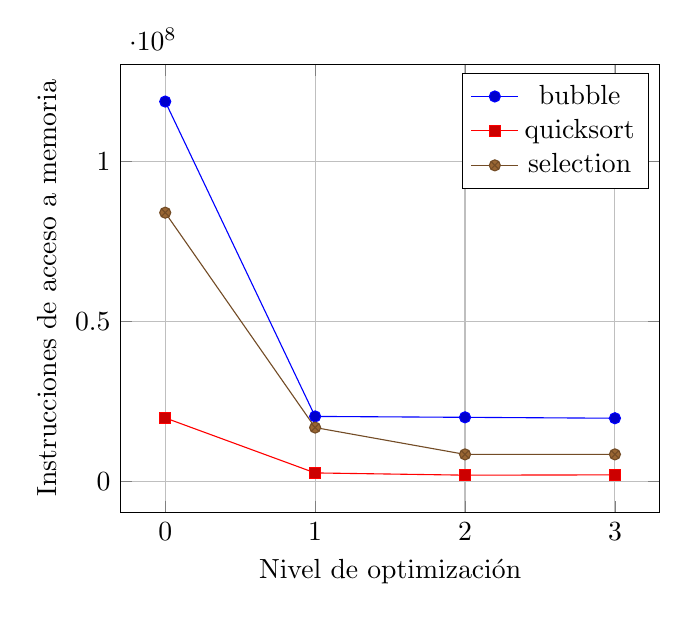
\begin{tikzpicture}
\begin{axis}[
xlabel=Nivel de optimización,
ylabel=Instrucciones de acceso a memoria,
grid=major,
xtick=data]
\addplot coordinates {
(0,118828473)
(1,20281490)
(2,19997926)
(3,19714362)
};
\addplot coordinates {
(0,19815975)
(1,2595975)
(2,1897211)
(3,1986973)
};
\addplot coordinates {
(0,84049617)
(1,16797696)
(2,8398848)
(3,8402944)
};
\legend{bubble,quicksort,selection}
\end{axis}
\end{tikzpicture}
\end{center}
\caption{Comparación de instrucciones de acceso a memoria entre funciones y optimizaciones.}
\label{graph:memoria}
\end{figure}

Si nos fijamos en la gráfica de la figura~\ref{graph:memoria}, vemos cómo en el nivel inicial de optimización hay número de accesos a memoria, que puede llegar a suponer alrededor de la mitad de las instrucciones totales de la funcion, reduciendose notablemente en los niveles superiores. Esta diferencia se debe, principalmente, al uso que se hace de los registros disponibles según el nivel de optimización. Por ejemplo, si vemos el código en ensamblador de \orden{bubble0} nos damos cuenta de que solamente hace uso de dos registros durante su ejecución: \orden{v0} y \orden{v1}. Por otro lado, en \orden{bubble1}, \orden{bubble2} y \orden{bubble3} se utilizan, no solo \orden{v0} y \orden{v1} sino también otros registros como \orden{a1}, \orden{a2} y \orden{a3}, aprovechando mejor los recursos disponibles en el procesador.

\begin{figure}[htbp]
\begin{center}
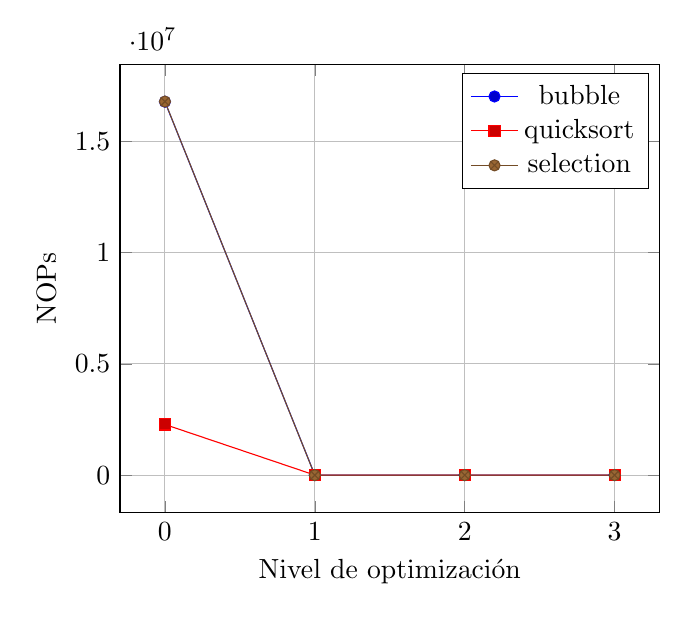
\begin{tikzpicture}
\begin{axis}[
xlabel=Nivel de optimización,
ylabel=NOPs,
grid=major,
xtick=data]
\addplot coordinates {
(0,16785411)
(1,4097)
(2,4097)
(3,4097)
};
\addplot coordinates {
(0,2278408)
(1,3403)
(2,0)
(3,0)
};
\addplot coordinates {
(0,16793603)
(1,1)
(2,1)
(3,1)
};
\legend{bubble,quicksort,selection}
\end{axis}
\end{tikzpicture}
\end{center}
\caption{Comparación de instrucciones \orden{nop} entre funciones y optimizaciones.}
\label{graph:nops}
\end{figure}
El número de instrucciones \orden{nop}, como se aprecia en la figura~\ref{graph:nops}, es considerablemente alto en las funciones cuyo nivel de optimización es `0', pero se reduce en el resto de los niveles de optimización, con respecto al más bajo. La cantidad de \orden{nop} en una función nos da una idea de la eficencia de la misma, ya que esta instrucción supone que el procesador no comienza una instrucción nueva en ese ciclo. El número es alto en el nivel inferior de optimización ya que el compilador no trata de reordenar las funciones para evitar dependencias entre ellas, lo que supone que el procesador deba esperar a que esté el dato disponible o a poder usar la unidad aritmético-lógica. Muchos de estos ciclos de espera también se producen después de las instrucciones de salto, en las funciones sin optimizar. Esto se debe a que no se puede realizar el salto hasta que no se haya calculado la dirección a la que se ha de ir, de ahí el \orden{nop} que podemos ver en el código desensamblado de todas las funciones sin optimizar detrás de este tipo de instrucciones. En los siguientes niveles, se aprovecha este espacio para colocar ahí una instrucción anterior a la de salto, siempre y cuando el resultado de esta función no sea determinante para calcular la dirección de destino del propio salto.

\subsection{Depuración y legibilidad del código.} % (fold)
\label{sub:Depuración y legibilidad del código.}
A partir del primer nivel de optimización el tamaño de la función y los tipos de instrucciones en ensamblador que podemos encontrar no varían mucho. Sin embargo sí que se producen reordenamiento de las instrucciones por parte del compilador para aprovechar mejor las unidades funcionales del microprocesador. Esto tiene la desventaja de que, a la hora de depurar el código ensamblado, es más difícil relacionar las instrucciones en lenguaje MIPS con las correspondientes en C.\@ Por ello, durante la fase de desarrollo del programa se debe mantener el nivel de optimización más bajo posible para facilitar la tarea de depuración.

Esto se puede observar en las funciones desensambladas del apéndice~\ref{chap:apendice4}. Por ejemplo, en las funciones que han sido compiladas usando el nivel de optimización `0', detrás de las instrucciónes de salto condicional siempre encontramos un \orden{nop}. Sin embargo, en el resto, debido a la opción \orden{-fdelayed-branch} encontramos en su lugar instrucciones que se ejecutarían antes si no se hubiese usado esta opción. Lo que puede dar lugar a confusión cuando se revisa el código (sobre todo si no se está familiarizado con estas optimizaciones y el modelo de programación de MIPS).

La desventaja de leer y depurar el código compilado sin optimizaciones es el exceso de movimientos entre el stack y los registros que se producen. Si acudimos otra vez al ejemplo de la función \orden{bubble0}, se puede ver cómo, durante toda la función, se guardan continuamente los valores de los registros \orden{v0} y \orden{v1} en el stack y, a continuación, se vuelven a leer. Esto no ocurre en el resto de funciones ya que en estas se hace más uso de los registros y menos del stack.
% subsection Depuración y legibilidad del código. (end)

\section{Análisis del tiempo de ejecución.} % (fold)
\label{sec:Análisis del tiempo de ejecución.}
Ya hemos visto el aspecto de las funciones en ensamblador, la cantidad de instrucciones en cada una de ellas y el tipo de instrucciones que las componen. Pero, ¿cómo se traducen estas diferencias en el rendimiento final de la aplicación? ¿hasta qué punto merece la pena el aumento de la complejidad del código ensamblador?.

Normalmente, el nivel de optimización con el que se compila un programa también afecta al propio tiempo de compilación del mismo. Debido al tamaño del programa del que aquí se trata (el archivo del programa del apartado anterior que se carga a la placa ocupa solamente 314~kB y su compilación tarda 3 segundos en mi portátil), este hecho se obvia al no tener un gran impacto en el proceso de creación de un programa para Chipkit o Arduino.

Hay varias formas de determinar el rendimiento de un programa o función. Podemos, por ejemplo, medir cuántos cálculos realiza por unidad de tiempo, pero esta medida no es adecuada para el este tipo de aplicación. En este caso lo que se intenta conseguir (en términos de rendimiento y optimización) es reducir el retardo que se produce desde que el usuario envía la órden hasta que obtiene la respuesta. Por lo que para saber el rendimiento de cada función y nivel de optimización, se usará el tiempo que tarda en ejecutarse dicha función, que será el tiempo de respuesta de la aplicación~\footnote{Cuando se ejecuta una órden este debe ser procesado, al igual que el vector de números que se pasa como parámetro, pero este tiempo será constante en todas las funciones al ser su código común a todas ellas.}.

\begin{figure}[htbp]
\begin{center}
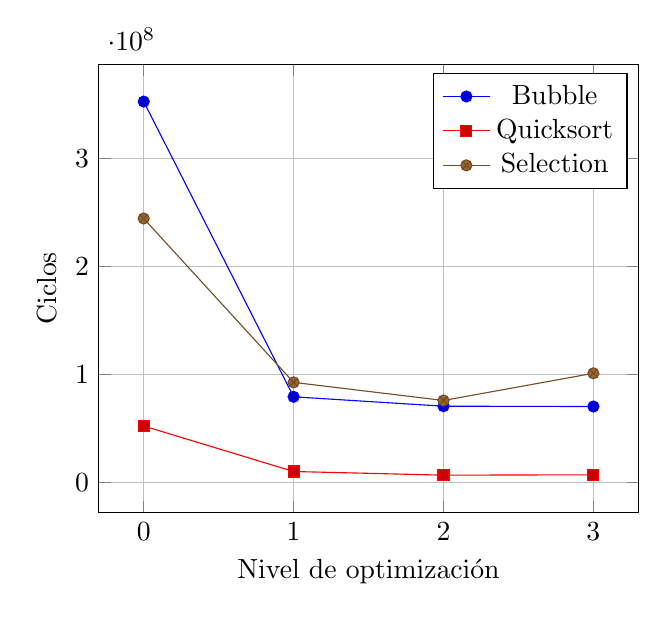
\begin{tikzpicture}
\begin{axis}[
xlabel=Nivel de optimización,
ylabel=Ciclos,
grid=major,
xtick=data]
\addplot coordinates {
	(0,352390396)
	(1,79200250)
	(2,70509212)
	(3,70225162)
};
\addplot coordinates {
	(0,	52175666)
	(1,	10090462)
	(2,	6713156)
	(3,	7025934)
};
\addplot coordinates {
	(0,	244191650)
	(1,	92569958)
	(2,	75805786)
	(3,	100967950)
};
\legend{Bubble,Quicksort,Selection}
\end{axis}
\end{tikzpicture}
\end{center}
\caption{Número de ciclos según función y optimización}
\label{graph:ciclos}
\end{figure}

En la figura~\ref{graph:ciclos} están representados la cantidad de ciclos de procesador que ha llevado ejecutar cada una de las funciones según el nivel de optimización. Se observa un patrón claro, al reducirse el tiempo de ejecución considerablemente cuando se utiliza el primer nivel de optimización, con respecto al inicial. Por ejemplo en el caso del algoritmo `Quick Sort' esta reducción supone un 80\% menos de ciclos tan solo eligiendo el primer nivel de optimización, siendo menor en los otros dos. Incluso en el nivel de optimización `0', este algoritmo ya es más rápido que cualquiera de los otros dos en el tercer nivel de optimización.

Si nos fijamos en la ganancia de rendimiento para niveles de optimización más altos que el primero, se puede ver que es muy inferior a la que se obtiene con el primer nivel (en comparación al nivel `0'). Este resultado es de esperar debido a que las optimizaciones que se llevan a cabo en los niveles superiores son más específicas y en estos algoritmos no tienen gran efecto. En el caso del algoritmo de selección, además, vemos como, no solo no se reduce el tiempo de ejecución al usar el tercer nivel de optimización, sino que aumenta con respecto al primer y segundo nivel. Este comportamiento no lo vemos en las otras funciones que, aunque muy limitada, si presentan una ganancia en el rendimiento final.
\begin{table}[htb]
	\begin{center}
		\begin{tabular}{lllll}
      \textbf{Algoritmo} & \textbf{Nivel 0} & \textbf{Nivel 1} & \textbf{Nivel 2} & \textbf{Nivel 3} \\
      \hline
      \textit{Bubble		}&	352390396	&	79200250 (77.52\%)	&	70509212 (10.97\%)	&	70225162 (0.4\%) \\
			\textit{QuickSort	}	&	52175666	&	10090462	(80.66\%)	&	6713156 (33.47\%)	&	7025934 (-4.66\%) \\
			\textit{Selection	} &	244191650	&	92569958 (62.09\%)	&	75805786 (18.11\%)	&	1009679 (-33.19\%) \\
		\end{tabular}
	\end{center}
\caption{Algoritmos y ciclos de ejecución. Ganancia con respecto al nivel anterior entre paréntesis.}
\label{tabla:ciclos}
\end{table}
% section Análisis del tiempo de ejecución. (end)
\section{Limitaciones de la biblioteca Arduino.} % (fold)
\label{sec:Limitaciones de la biblioteca Arduino.}

La plataforma Arduino, incluyendo Chipkit, está pensada para poder crear programas sin tener que conocer el funcionamiento interno de cada microcontrolador. Es una capa de abstracción más, que permite usar las mismas funciones o incluso programas en microcontroladores diferentes. Por ejemplo, si ejecutamos la función \orden{digitalWrite(13, HIGH)} sabemos que se encenderá el LED de usuario que tienen instalado todas las placas convencionales compatibles con Arduino. No es necesario conocer a que puerto del microcontrolador está conectado dicho LED, que varía según el modelo de placa. Por ejemplo, en el chipKIT MAX32 este LED (LD4) se encuentra conectado al tercer pin del puerto A, sin embargo, en el chipKIT Uno32 lo encontramos el el sexto pin del puerto G.\@

Cuando queremos leer un valor en una de las entradas analógicas ocurre algo similar: a la función \orden{analogRead()} solo hay que pasarle el pin de la placa, cuyo número se encuentra impreso al lado del mismo y la función se encarga de realizar toda la configuración necesaria para obtener el valor del ADC.\@

Esta simplificación tiene un precio. Cada vez que se quiere leer o escribir en cada uno de estos puertos, la función encargada de hacerlo lleva a cabo la configuración y la posterior lectura o escritura. Esta sobrecarga hace que cualquiera de estas operaciones sea considerablemente más lenta que si se realizara con funciones de más bajo nivel o accediendo directamente a los registros.

Para ilustrar la diferencia he medido de dos formas distintas la frequencia a la que es capaz el Chipkit Max32 de cambiar el estado de un pin de salida. Usando la funcion de Arduino para escribir en una salida digital (\orden{digitalWrite()}) y accediendo a los registros directamente he generado dos ondas cuadradas de diferentes frecuencias. La primera forma de medir la diferencia ha sido usando un método similar al que usamos en el apartado anterior: guardando el valor del contador del microprocesador antes y después de la ejecución de lo que se desea medir. En este caso he optado por medir el tiempo que tarda en ejecutarse un bucle `for' en el que se pone a alto y bajo un pin del microcontrolador. El bucle se repite \(10^5\) veces.

\begin{table}[htb]
	\begin{center}
		\begin{tabular}{llllll}
      \textbf{Método}		&		\textbf{Cuentas}		&		\textbf{Ciclos}		&		\textbf{Ciclos/iteración}	&		\textbf{Periodo}		&		\textbf{Frecuencia} \\
			\hline
      \textit{Arduino}		&		5763684		&		11527368	&		115.27						&		1.44 us		&		694 kHz \\
      \textit{Registros}	&		501040		&		1002080		&		10.02							&		125.26 ns	&		7.98 MHz \\

		\end{tabular}
	\end{center}
	\caption{Diferencia entre \orden{digitalWrite()} y acceso directo al registro usando un bucle \orden{for} de $10^5$ iteraciones y midendo el tiempo que tarda en completarse este bucle.}
	\label{ard_vs_reg:1}
\end{table}

En la figura~\ref{ard_vs_reg:1} se puede apreciar la diferencia de velocidad cuando se realiza la escritura digital en un puerto dependiendo del método empleado. Según estos datos el acceso directo a los registros del microcontrolador nos otorga la posibilidad de ejecutar esta operación a una frecuencia un orden de magnitud mayor que con la función \orden{digitalWrite()} de la biblioteca Arduino. Para contrastar los resultados también he obtado por realizar las mediciones con otro método. Usando un bucle infinito con \orden{while(1)} he medido la frecuencia de la onda cuadrada que se genera en el pin correspondiente y, como se puede ver en la figura~\ref{ard_vs_reg:2} los resultados son muy similares al primer método.

\begin{table}[htb]
	\begin{center}
		\begin{tabular}{ll}
      \textbf{Método}		&		\textbf{Frecuencia}	\\
			\hline
      \textit{Arduino}		&		700 kHz			\\
      \textit{Registros}	&		7.983	MHz		\\
		\end{tabular}
	\end{center}
	\caption{Frecuencia de conmutación según el método empleado. Medida usando un multímetro UNI-T UT61E}
	\label{ard_vs_reg:2}
\end{table}

Esta diferencia de velocidad dependiendo del método empleado es debida a que las funciones de la biblioteca Arduino no se encargan solo de, por ejemplo, escribir en un pin digital, también comprueban que el pin existe y en el caso de existir, a que puerto del microcontrolador pertenece. Como el objetivo de la biblioteca Arduino no es solo simplificar funciones comunes en microcontroladores, sino también generar código portable, es decir, código que pueda ser compilado en diferentes microcontroladores, las funciones deben ser capaces de ejecutarse teniendo en cuenta esto. Cuando usamos registros la velocidad aumenta, como ya he dicho, a expensas de reducir la legibilidad del código y su portabilidad.

Otra limitación de Arduino es la falta de funciones para controlar características de cada microcontrolador, como por ejemplo interrupciones y temporizadores. Si queremos hacer uso de alguna de estas características no queda más remedio que acudir a las funciones del fabricante o directamente a los registros del microcontrolador. Otro ejemplo de este tipo de limitación está presente en el programa escrito para la siguiente sección. En este programa se muestrea de forma regular (a 8 kHz) una entrada analógica. Esto no es posible realizarlo con la función de Arduino \orden{analogRead()} ya que es demasiado lenta, al tener que configurar cada vez el pin de entrada. Usando los registros del microcontrolador podemos configurar el ADC para que tome muestras de forma regular~\footnote{En el caso del chip que incorpora el Chipkit Max32 se pueden alcanzar frecuencias de muestreo de 1 Msps.} y autónoma, generando una interrupción cuando la muestra está lista.
% section Limitaciones de la biblioteca Arduino. (end)

\section{Ejemplo de aplicación relacionada con la carrera de telecomunicación.} % (fold)
\label{sec:Ejemplo de aplicación relacionada con la carrera de telecomunicación.}
% section Ejemplo de aplicación relacionada con la carrera de telecomunicación. (end)

Para finalizar, he decidido escribir una aplicación relacionada con el área de las telecumicaciones. He optado por recrear un programa que elaboré como trabajo final en la asignatura `Laboratorio de tratamiento digital de la señal'. Se trata de un detector de tonos mediante el uso del algoritmo de Goertzel. El programa que desarrollé durante la asignatura funcionaba en un DSP, más concretamente se trataba de un Analog Devices ADSP-2181~\footnote{www.analog.com/en/processors-dsp/adsp-21xx/adsp-2181/products/product.html}.
\begin{figure}[htb]
\centering
\begin{tikzpicture}
	\matrix[row sep=15mm, column sep=25mm]
	{
		\node[dspnodeopen,dsp/label=left]	(m00)	{$x[n]$};	&
		\node[dspadder]						(m01)	{};			&
		\node[dspnodeopen]					(m02)	{$v_k[n]$}; &
		\node[dspadder]						(m03)	{};			&
		\node[dspnodeopen,dsp/label=right]	(m04)	{$y[n]$}; 	\\

		\node[coordinate]					(m10)	{};			&
		\node[dspadder]						(m11)	{};			&
		\node[coordinate]					(m12)	{};			&
		\node[coordinate]					(m13)	{};			\\

		\node[coordinate]					(m20)	{};			&
		\node[coordinate]					(m21)	{};			&
		\node[coordinate]					(m22)	{};			\\
	};

	\foreach \i [evaluate = \i as \j using int(\i+1)] in {0,1,2,3}
		\draw[dspflow] (m0\i) -- (m0\j);

	\draw[dspflow] (m11) -- (m01);
	\draw[dspflow] (m02) -- node[midway,right] {$\z^{-1}$} (m12);
	\draw[dspflow] (m12) -- node[midway,above] {$2cos(2\pi{}k/N)$} (m11);
	\draw[dspflow] (m12) -- node[midway,below] {$-W_{n^{k}}$} (m13);
	\draw[dspflow] (m13) -- (m03);
	
	\draw[dspflow] (m12) -- node[midway,right] {$\z^{-1}$} (m22);
	\draw[dspflow] (m22) -- node[midway,above] {$-1$} (m21);
	\draw[dspflow] (m21) -- (m11);

\end{tikzpicture}
\caption{Algoritmo de Goertzel.}
\label{goertzel}
\end{figure}

El DSP tomaba muestras con una frecuencia de muestreo de 8 kHz, que es la misma que he usado en este programa. Normalmente un DSP toma una muestra y realiza el procesado que requiera el algoritmo en dicha muestra. Este programa hace uso de la posibilidad que tienen los ADC de este microcontrolador de realizar el muestreo automáticamente. De esta forma, una vez configurado, solo hay que escribir una función que se encargue de recoger la muestra cuando el ADC genera una interrupción y decidir cuando empieza y acaba el automuestreo. Las funciones que gestionan una interrupción deben ser lo más cortas posibles, por lo que en las primeras revisiones del programa, esta función se encargaba solomente de almacenar la muestra en un vector y aumentar el contador de muestras. Una vez estan todas las muestras almacenadas, se para el automuestreo y comienza el procesado de los datos en la función \orden{loop()}. Cabe mencionar que este muestreo automático y regular no es posible implementarlo usando tan solo las funciones de la biblioteca Arduino, por lo que es necesario recurrir al manual del microcontrolador y a sus registros para llevarlo a cabo.

Este programa toma las muestras a la misma frecuencia que el DSP de prácticas~\footnote{Aunque, de acuerdo a las especificaciones del PIC32MX795F512L, es capaz de alcanzar frecuencias de muestreo de 1 MHz.}. Viendo el número de operaciones y su complejidad decidí implementarlas directamente en la función de interrupción del ADC, al haber tiempo suficiente entre interrupciones para realizar las operaciones que requiere cada muestra. Con esto logré un funcionamiento idéntico al programa del DSP.\@

Durante las primeras revisiones del programa, todas las operaciones matemáticas que el algoritmo requiere se realizaban usando variables de tipo \orden{float}, es decir, de coma flotante. Como ya comenté en el apartado dedicado al PIC32MX795F512L, este chip no dispone de unidad de coma flotante. Como consecuencia, todas las operaciones sobre variables de este tipo deben ser emuladas mediante el uso de una biblioteca. Realizar las operaciones de este modo consume muchos ciclos del procesador, lo que imposibilitaba el mover las operaciones que se realizaban en cada muestra a la función que gestiona las interrupciones.

Para aumentar la velocidad del programa, decidí usar coma fija. Debido a la naturaleza de las muestras obté por representar con 16 bits el rango de -1 a 1 que, convertido a este formato sería -32767 a 32767 (\(-2^{15}+1\) a \(2^{15}-1\)). Con 16 bits tenemos suficiente precisión ya que las muestras que toma el ADC son de 10 bits y además tenemos la posibilidad de multiplicar dos de estos números y obtener uno de 32 bits que, al ser este el tamaño de palabra del procesador, las operaciones no requeriran más de un ciclo. Para convertir los datos del ADC a esta representación tan solo hace falta realizar un desplazamiento, al igual que para reducir los números de 32 bits a 16. La ventaja de esto en lugar de haber multiplicado por una potencia de 10 los números es que los desplazamientos se ejecutan en un ciclo.

% Goertzel y Filtros Digitales
% Muestreo
% Procesamiento de cada muestra y procesamiento final

\subsubsection{Análisis de rendimiento}

A grandes rasgos, podemos dividir el funcionamiento del programa en dos partes: la recursiva y una parte final. En este caso la parte recursiva del programa es el procesamiento que se realiza de cada muestra recogida y convertida por el ADC del microcontrolador. La frecuencia de muestreo se verá principalmente limitada por este procesamiento de cada muestra, ya que he elegido realizarlo nada más obtenerla para imitar lo mas fielmente posible el funcionamiento de un DSP\@. Como alternativa, se pueden guardar todas las muestras en un vector y, una vez llenado, iterar sobre este realizando el procesado de todas las muestras.

Cada uno de los dos métodos tiene sus ventajas. Si optamos por usar el primero, de forma similar a un DSP, el tiempo en el que se obtiene un resultado al finalizar el muestreo será menor, suponiendo que la frecuencia de muestreo sea tal que permita el correcto procesamiento de cada muestra entre muestreos. La ventaja del segundo método es que, al no tener que realizar el procesamiento entre muestreos podemos reducir el tiempo entre ellos y por lo tanto aumentar su frecuencia, lo que en este caso nos permitiría, por ejemplo, detectar frecuencias mayores al primer método.

\begin{minipage}{\linewidth}
\begin{lstlisting}
extern "C"
{
  void __ISR(_ADC_VECTOR, ipl6) ADCInterruptHandler()
  {
    IFS1CLR = 2;
    /* Normaliza la muestra y la atenua para evitar la saturacion
       al final del filtro. */
    int muestra = ADC1BUF0;
    muestra = muestra - 512;
    muestra = muestra << (GAIN_BITS - 9);
    muestra *= ATENUADOR;
    muestra >>= GAIN_BITS;
    
    /* Guardamos el valor maximo de las muestras */
    if(abs(muestra) > abs(max)) {
      max = muestra;
    }

    /* Parte recursiva de Goertzel */
    q0 = (COSENO * q1);
    q0 -= (MITAD * q2);
    q0 += (COSENO * q1);
    q0 -= (MITAD * q2);
    q0 >>= GAIN_BITS;
    q0 += muestra;
    q2 = q1;
    q1 = q0;

    /* Aumentamos el valor del contador de muestras */
    contador_muestras++;

    /* Si tenemos todas las muestras, cancelamos el
       automuestreo para llevar a cabo la parte 
       final del algoritmo */
    if(contador_muestras >= N_MUESTRAS)
    {
      contador_muestras = 0;
      muestras_listas = true;
      AD1CON1bits.ASAM = 0; // Paramos el automuestreo
    }
  }
}
\end{lstlisting}
\end{minipage}

Este código es el que se ejecuta cada vez que el ADC ha terminado de convertir una muestra~\footnote{El microcontrolador está configurado para que realice el muestreo y la conversión de forma automática con una frecuencia de 8kHz, interrumpiendo cuando se haya completado.}, por lo que es la parte que más interesa analizar para conocer el rendimiento final. Se puede dividir en aproximadamente tres partes. En la primera se obtiene el valor guardado en el registro del ADC, se normaliza, se le aplica una atenuación para evitar saturar el filtro y se guarda el valor máximo para compararlo al final con el valor que devuelve el algoritmo. En la segunda parte se realiza la parte recursiva del algoritmo sobre la muestra actual. Por último, se controla la cantidad de muestras que se han procesado y, en el caso de estar todas, se para el automuestreo para comenzar el procesamiento final en la parte principal del programa.

\begin{figure}[htb]
  \begin{minipage}{.45\textwidth}
\begin{lstlisting}[language={[mips]Assembler},basicstyle=\ttfamily\scriptsize]
 0:	415de800  rdpgpr	sp,sp
 4:	401a7000  mfc0	k0,c0_epc
 8:	401b6000  mfc0	k1,c0_status
 c:	27bdffe8  addiu	sp,sp,-24
10:	afbb0010  sw	k1,16(sp)
14:	7c1b7844  ins	k1,zero,0x1,0xf
18:	377b1800  ori	k1,k1,0x1800
1c:	afba0014  sw	k0,20(sp)
20:	409b6000  mtc0	k1,c0_status
24:	afa30008  sw	v1,8(sp)
28:	afa20004  sw	v0,4(sp)
2c:	24030002  li	v1,2
30:	3c020000  lui	v0,0x0
34:	ac430000  sw	v1,0(v0)
38:	97820000  lhu	v0,0(gp)
3c:	3c030000  lui	v1,0x0
40:	8c630000  lw	v1,0(v1)
44:	afa4000c  sw	a0,12(sp)
48:	3042ffff  andi	v0,v0,0xffff
4c:	3c040000  lui	a0,0x0
50:	00021080  sll	v0,v0,0x2
54:	24840000  addiu	a0,a0,0
58:	00441021  addu	v0,v0,a0
5c:	ac430000  sw	v1,0(v0)
60:	3c020000  lui	v0,0x0
64:	24030004  li	v1,4
68:	ac430000  sw	v1,0(v0)
\end{lstlisting}
\end{minipage}
\hfill
\begin{minipage}{.45\textwidth}
\begin{lstlisting}[language={[mips]Assembler},basicstyle=\ttfamily\scriptsize]
6c:	97820000  lhu	v0,0(gp)
70:	24420001  addiu	v0,v0,1
74:	3042ffff  andi	v0,v0,0xffff
78:	a7820000  sh	v0,0(gp)
7c:	97820000  lhu	v0,0(gp)
80:	3042ffff  andi	v0,v0,0xffff
84:	2c4212ca  sltiu	v0,v0,4810
88:	14400007  bnez	v0,a8
8c:	24030001  li	v1,1
90:	a7800000  sh	zero,0(gp)
94:	3c020000  lui	v0,0x0
98:	a3830000  sb	v1,0(gp)
9c:	8c430000  lw	v1,0(v0)
a0:	7c031084  ins	v1,zero,0x2,0x1
a4:	ac430000  sw	v1,0(v0)
a8:	8fa4000c  lw	a0,12(sp)
ac:	8fa30008  lw	v1,8(sp)
b0:	8fa20004  lw	v0,4(sp)
b4:	41606000  di
b8:	000000c0  ehb
bc:	8fba0014  lw	k0,20(sp)
c0:	8fbb0010  lw	k1,16(sp)
c4:	409a7000  mtc0	k0,c0_epc
c8:	27bd0018  addiu	sp,sp,24
cc:	41dde800  wrpgpr	sp,sp
d0:	409b6000  mtc0	k1,c0_status
d4:	42000018  eret
 \end{lstlisting}
 \end{minipage}
 \caption{Parte recursiva de Goertzel desensamblada (Segundo nivel de optimización)}
 \label{goertzel_recursivo_ensamblador}
 \end{figure}
 En la figura~\ref{goertzel_recursivo_ensamblador} se encuentra el código que se muestra antes desensambado usando \programa{pic32-objdump} de la misma forma que he hecho con el código del otro programa. Al igual que en el apartado anterior, he contado el número de instrucciones según el tipo y optimización. Debido a la diferente naturaleza de este programa, en vez de contar el número de instrucciones al finalizar la ejecución, he contado el número en una de las iteraciones intermedias de esta parte, es decir, cuando la última parte se evalúa como falsa y no se ejecuta. En la tabla~\ref{tabla:tiempos_goertzel} se puede observar el número de instrucciones obtenido junto con el tiempo que ha llevado ejecutarlas.

\begin{table}[htb]
	\begin{center}
		\begin{tabular}{llll}
			\textbf{Nivel} & \textbf{Ciclos} & \textbf{Tiempo} & \textbf{Instrucciones} \\
			\hline
			\textit{O0} & 114 & \(1.43\mu s\) & 128 \\
			\textit{O1} & 82 & \(1.03\mu s\) & 101 \\
			\textit{O2} & 82 & \(1.03\mu s\) & 100 \\
			\textit{O3} & 82 & \(1.03\mu s\) & 100 \\
		\end{tabular}
		\caption{Tiempos de ejecución de la parte recursiva del programa}
		\label{tabla:tiempos_goertzel}
	\end{center}
\end{table}

La diferencia entre los distintos niveles de optimización es prácticamente despreciable en este caso. Debido a la frecuencia de muestreo de 8kHz que he usado en el programa para simular el DSP usado en clase, el tiempo que hay disponible entre muestras para realizar procesamiento es suficientemente largo como para que no importe el nivel de optimización elegido, para esta aplicación en particular. Con esta frecuencia disponemos de alrededor de \(125\mu s\) entre muestras, mientras que en el peor de los casos (sin optimización) el procesamiento de la muestra solo tarda \(1.43\mu s\).

De hecho, sería posible ejecutar este algoritmo 8 veces de forma simultánea, es decir, realizar ocho procesados distintos de muestra entre muestreos, de forma que podemos, por ejemplo, calcular el dígito marcado en un teléfono analógico (si conectáramos la salida del teléfono a la entrada analógica del microcontrolador) o de cualquier otro dispositivo que generase código de marcación por tonos. 


\chapter{Conclusiones}
En este capítulo expondré las conclusiones obtenidas durante la elaboración de este trabajo. Se subdivide en dos apartados: conclusiones técnicas, donde comentaré los resultados de las mediciones y el proceso usado para obtenerlas; conclusiones personales, donde expondré mis pensamientos acerca de este trabajo junto con las cosas que he podido aprender durante la realización del mismo.

\subsection{Conclusiones técnicas}
Este trabajo tenía diferentes objetivos. El primero de ellos era analizar el proceso de compilación, enlazado y carga en la placa que lleva a cabo el IDE de Microchip (\programa{MPIDE}) de forma transparente al usuario. Una vez conocido este proceso había que desarrollar un método alternativo que me permitiera más transparencia y flexibilidad. Usando la opción de mostrar las órdenes ejecutadas en \programa{MPIDE} pude ver los programas a los que llama y en que orden. A partir de esta información ideé un archivo \orden{Makefile} que realizara las mismas acciones y que diese como resultado el programa cargado en la placa. Más tarde expandí la idea de un archivo Makefile a la creación de una plantilla de programa, es decir, una organización de carpetas en las que organizar las bibliotecas de terceros que pueda necesitar el programa, el código fuente y el ejecutable final. Fue interesante comprobar como había algunas acciones que el IDE llevaba a cabo antes de comenzar la compilación. A la hora de escribir un sketch en \programa{MPIDE} no es necesario declarar las funciones auxuiliares que pueda requerir la aplicación, a diferencia de como se haría en un programa normal escrito en C o C++. El IDE hace esta labor por el usuario, buscando las funciones que se hayan escrito en el sketch y añadiendo su definición al principio del mismo antes de comenzar la compilación. A parte de esto también añade un `include' con el archivo de cabecera que contiene todas las definiciones de las funciones de la biblioteca `core'.

El segundo objetivo planteado era comparar el efecto de los distintos niveles de optimización tenían sobre el rendimiento final del programa. Para esto se proponía la creación de un programa en el que se pudiese realizar esta comparación.

Una vez hecho esto, el siguiente objetvio era poner de manifiesto las limitaciones de la biblioteca Arduino frente a funciones de más bajo nivel que el fabricante provea en una biblioteca o directamente usando los registros del procesador y de periféricos.

Por último, se proponía la creación de un programa que pusiese en práctica conocimientos adquiridos durante la carrera. El programa tendría como objetivo detectar la presencia de un tono en una entrada analógica cuya señal se obtendría con un micrófono.


\backmatter % Apéndices, bibliografia ...


\clearpage
\addcontentsline{toc}{chapter}{Bibliografia y referencias}
\bibliographystyle{plain}
\bibliography{bibliografia}


\addcontentsline{toc}{chapter}{Software usado}
\chapter*{Software utilizado}
% -*-programas.tex-*-
% Este fichero es parte de la plantilla LaTeX para
% la realización de Proyectos Final de Carrera, protejido
% bajo los términos de la licencia GFDL.
% Para más información, la licencia completa viene incluida en el
% fichero fdl-1.3.tex

% Copyright (C) 2009 Pablo Recio Quijano 
Para la realización de esta memoria he utilizado diferentes programas.

\section*{Vim}
\programa{Vim} es uno de los editores de texto más utilizado en entornos Unix, enfocado en programación. La ventaja de usar este editor es que está preinstalado en cualquier sistema Unix (puede estar instalado Vim o Vi) y es altamente personalizable mediante su archivo de configuración y con plugins.

\section*{Sublime Text + Latexing}
Otro editor de textos que he utilizado para la creación de esta memoria es \programa{Sublime Text} que, a diferencia de \programa{Vim}, es de pago. Al igual que \programa{Vim} es posible ampliar su funcionalidad con plugins.

\section*{Git}
Para mantener un control de versiones he optado por utilizar \programa{Git}. Con \programa{Git} puedo, no solo guardar las versiones, sino también crear diferentes ramas o utilizar un servicio como Github.com, que me permite almacenar tanto esta memoria como los programas que he creado para este trabajo.

\section*{GNU Make}

\programa{GNU Make} es el programa de recompilación y de control de
dependencias por excelencia. Se puede utilizar para compilar proyectos
software en diversos códigos, o como en el caso de este documento,
para compilar documentos \LaTeX{} con diversas opciones.\\

Para más información \cite{pdf:make}


%\addcontentsline{toc}{chapter}{Apéndice 1: Resultado de la compilación en \programa{MPIDE}}
\appendix
\chapter{Apéndice 1: Resultado de la compilación en \programa{MPIDE}}\label{chap:apendice1}
\begin{lstlisting}[language=bash, label=bash:mpidecompilado, basicstyle=\small, breaklines=true]

/Applications/mpide.app/Contents/Resources/Java/hardware/pic32/compiler/pic32-tools/bin/pic32-g++  -O2  -c  -mno-smart-io  -w  -fno-exceptions  -ffunction-sections  -fdata-sections  -g  -mdebugger  -Wcast-align  -fno-short-double  -mprocessor=32MX795F512L  -DF_CPU=80000000L  -DARDUINO=23  -D_BOARD_MEGA_    -DMPIDEVER=0x01000305  -DMPIDE=23      -I/Applications/Mpide.app/Contents/Resources/Java/examples/1.Basics/Blink   -I/Applications/Mpide.app/Contents/Resources/Java/hardware/pic32/cores/pic32   -I/Applications/Mpide.app/Contents/Resources/Java/hardware/pic32/variants/Max32    /var/folders/f0/q5xc0_tj4jv4ljd_lfz4pg5h0000gn/T/build2117742867436922308.tmp/Blink.cpp  -o  /var/folders/f0/q5xc0_tj4jv4ljd_lfz4pg5h0000gn/T/build2117742867436922308.tmp/Blink.cpp.o
/Applications/mpide.app/Contents/Resources/Java/hardware/pic32/compiler/pic32-tools/bin/pic32-g++  -O2  -g1  -c  -mprocessor=32MX795F512L  -DF_CPU=80000000L  -DARDUINO=23  -D_BOARD_MEGA_    -DMPIDEVER=0x01000305  -DMPIDE=23      -I/Applications/Mpide.app/Contents/Resources/Java/hardware/pic32/cores/pic32   -I/Applications/Mpide.app/Contents/Resources/Java/hardware/pic32/variants/Max32    /Applications/Mpide.app/Contents/Resources/Java/hardware/pic32/cores/pic32/cpp-startup.S  -o  /var/folders/f0/q5xc0_tj4jv4ljd_lfz4pg5h0000gn/T/build2117742867436922308.tmp/cpp-startup.S.o
/Applications/mpide.app/Contents/Resources/Java/hardware/pic32/compiler/pic32-tools/bin/pic32-g++  -O2  -g1  -c  -mprocessor=32MX795F512L  -DF_CPU=80000000L  -DARDUINO=23  -D_BOARD_MEGA_    -DMPIDEVER=0x01000305  -DMPIDE=23      -I/Applications/Mpide.app/Contents/Resources/Java/hardware/pic32/cores/pic32   -I/Applications/Mpide.app/Contents/Resources/Java/hardware/pic32/variants/Max32    /Applications/Mpide.app/Contents/Resources/Java/hardware/pic32/cores/pic32/crti.S  -o  /var/folders/f0/q5xc0_tj4jv4ljd_lfz4pg5h0000gn/T/build2117742867436922308.tmp/crti.S.o
/Applications/mpide.app/Contents/Resources/Java/hardware/pic32/compiler/pic32-tools/bin/pic32-g++  -O2  -g1  -c  -mprocessor=32MX795F512L  -DF_CPU=80000000L  -DARDUINO=23  -D_BOARD_MEGA_    -DMPIDEVER=0x01000305  -DMPIDE=23      -I/Applications/Mpide.app/Contents/Resources/Java/hardware/pic32/cores/pic32   -I/Applications/Mpide.app/Contents/Resources/Java/hardware/pic32/variants/Max32    /Applications/Mpide.app/Contents/Resources/Java/hardware/pic32/cores/pic32/crtn.S  -o  /var/folders/f0/q5xc0_tj4jv4ljd_lfz4pg5h0000gn/T/build2117742867436922308.tmp/crtn.S.o
/Applications/mpide.app/Contents/Resources/Java/hardware/pic32/compiler/pic32-tools/bin/pic32-gcc  -O2  -c  -mno-smart-io  -w  -ffunction-sections  -fdata-sections  -g  -mdebugger  -Wcast-align  -fno-short-double  -mprocessor=32MX795F512L  -DF_CPU=80000000L  -DARDUINO=23  -D_BOARD_MEGA_    -DMPIDEVER=0x01000305  -DMPIDE=23      -I/Applications/Mpide.app/Contents/Resources/Java/hardware/pic32/cores/pic32   -I/Applications/Mpide.app/Contents/Resources/Java/hardware/pic32/variants/Max32    /Applications/Mpide.app/Contents/Resources/Java/hardware/pic32/cores/pic32/exceptions.c  -o  /var/folders/f0/q5xc0_tj4jv4ljd_lfz4pg5h0000gn/T/build2117742867436922308.tmp/exceptions.c.o
/Applications/mpide.app/Contents/Resources/Java/hardware/pic32/compiler/pic32-tools/bin/pic32-gcc  -O2  -c  -mno-smart-io  -w  -ffunction-sections  -fdata-sections  -g  -mdebugger  -Wcast-align  -fno-short-double  -mprocessor=32MX795F512L  -DF_CPU=80000000L  -DARDUINO=23  -D_BOARD_MEGA_    -DMPIDEVER=0x01000305  -DMPIDE=23      -I/Applications/Mpide.app/Contents/Resources/Java/hardware/pic32/cores/pic32   -I/Applications/Mpide.app/Contents/Resources/Java/hardware/pic32/variants/Max32    /Applications/Mpide.app/Contents/Resources/Java/hardware/pic32/cores/pic32/HardwareSerial_cdcacm.c  -o  /var/folders/f0/q5xc0_tj4jv4ljd_lfz4pg5h0000gn/T/build2117742867436922308.tmp/HardwareSerial_cdcacm.c.o
/Applications/mpide.app/Contents/Resources/Java/hardware/pic32/compiler/pic32-tools/bin/pic32-gcc  -O2  -c  -mno-smart-io  -w  -ffunction-sections  -fdata-sections  -g  -mdebugger  -Wcast-align  -fno-short-double  -mprocessor=32MX795F512L  -DF_CPU=80000000L  -DARDUINO=23  -D_BOARD_MEGA_    -DMPIDEVER=0x01000305  -DMPIDE=23      -I/Applications/Mpide.app/Contents/Resources/Java/hardware/pic32/cores/pic32   -I/Applications/Mpide.app/Contents/Resources/Java/hardware/pic32/variants/Max32    /Applications/Mpide.app/Contents/Resources/Java/hardware/pic32/cores/pic32/HardwareSerial_usb.c  -o  /var/folders/f0/q5xc0_tj4jv4ljd_lfz4pg5h0000gn/T/build2117742867436922308.tmp/HardwareSerial_usb.c.o
/Applications/mpide.app/Contents/Resources/Java/hardware/pic32/compiler/pic32-tools/bin/pic32-gcc  -O2  -c  -mno-smart-io  -w  -ffunction-sections  -fdata-sections  -g  -mdebugger  -Wcast-align  -fno-short-double  -mprocessor=32MX795F512L  -DF_CPU=80000000L  -DARDUINO=23  -D_BOARD_MEGA_    -DMPIDEVER=0x01000305  -DMPIDE=23      -I/Applications/Mpide.app/Contents/Resources/Java/hardware/pic32/cores/pic32   -I/Applications/Mpide.app/Contents/Resources/Java/hardware/pic32/variants/Max32    /Applications/Mpide.app/Contents/Resources/Java/hardware/pic32/cores/pic32/pins_arduino.c  -o  /var/folders/f0/q5xc0_tj4jv4ljd_lfz4pg5h0000gn/T/build2117742867436922308.tmp/pins_arduino.c.o
/Applications/mpide.app/Contents/Resources/Java/hardware/pic32/compiler/pic32-tools/bin/pic32-gcc  -O2  -c  -mno-smart-io  -w  -ffunction-sections  -fdata-sections  -g  -mdebugger  -Wcast-align  -fno-short-double  -mprocessor=32MX795F512L  -DF_CPU=80000000L  -DARDUINO=23  -D_BOARD_MEGA_    -DMPIDEVER=0x01000305  -DMPIDE=23      -I/Applications/Mpide.app/Contents/Resources/Java/hardware/pic32/cores/pic32   -I/Applications/Mpide.app/Contents/Resources/Java/hardware/pic32/variants/Max32    /Applications/Mpide.app/Contents/Resources/Java/hardware/pic32/cores/pic32/task_manager.c  -o  /var/folders/f0/q5xc0_tj4jv4ljd_lfz4pg5h0000gn/T/build2117742867436922308.tmp/task_manager.c.o
/Applications/mpide.app/Contents/Resources/Java/hardware/pic32/compiler/pic32-tools/bin/pic32-gcc  -O2  -c  -mno-smart-io  -w  -ffunction-sections  -fdata-sections  -g  -mdebugger  -Wcast-align  -fno-short-double  -mprocessor=32MX795F512L  -DF_CPU=80000000L  -DARDUINO=23  -D_BOARD_MEGA_    -DMPIDEVER=0x01000305  -DMPIDE=23      -I/Applications/Mpide.app/Contents/Resources/Java/hardware/pic32/cores/pic32   -I/Applications/Mpide.app/Contents/Resources/Java/hardware/pic32/variants/Max32    /Applications/Mpide.app/Contents/Resources/Java/hardware/pic32/cores/pic32/WInterrupts.c  -o  /var/folders/f0/q5xc0_tj4jv4ljd_lfz4pg5h0000gn/T/build2117742867436922308.tmp/WInterrupts.c.o
/Applications/mpide.app/Contents/Resources/Java/hardware/pic32/compiler/pic32-tools/bin/pic32-gcc  -O2  -c  -mno-smart-io  -w  -ffunction-sections  -fdata-sections  -g  -mdebugger  -Wcast-align  -fno-short-double  -mprocessor=32MX795F512L  -DF_CPU=80000000L  -DARDUINO=23  -D_BOARD_MEGA_    -DMPIDEVER=0x01000305  -DMPIDE=23      -I/Applications/Mpide.app/Contents/Resources/Java/hardware/pic32/cores/pic32   -I/Applications/Mpide.app/Contents/Resources/Java/hardware/pic32/variants/Max32    /Applications/Mpide.app/Contents/Resources/Java/hardware/pic32/cores/pic32/wiring.c  -o  /var/folders/f0/q5xc0_tj4jv4ljd_lfz4pg5h0000gn/T/build2117742867436922308.tmp/wiring.c.o
/Applications/mpide.app/Contents/Resources/Java/hardware/pic32/compiler/pic32-tools/bin/pic32-gcc  -O2  -c  -mno-smart-io  -w  -ffunction-sections  -fdata-sections  -g  -mdebugger  -Wcast-align  -fno-short-double  -mprocessor=32MX795F512L  -DF_CPU=80000000L  -DARDUINO=23  -D_BOARD_MEGA_    -DMPIDEVER=0x01000305  -DMPIDE=23      -I/Applications/Mpide.app/Contents/Resources/Java/hardware/pic32/cores/pic32   -I/Applications/Mpide.app/Contents/Resources/Java/hardware/pic32/variants/Max32    /Applications/Mpide.app/Contents/Resources/Java/hardware/pic32/cores/pic32/wiring_analog.c  -o  /var/folders/f0/q5xc0_tj4jv4ljd_lfz4pg5h0000gn/T/build2117742867436922308.tmp/wiring_analog.c.o
/Applications/mpide.app/Contents/Resources/Java/hardware/pic32/compiler/pic32-tools/bin/pic32-gcc  -O2  -c  -mno-smart-io  -w  -ffunction-sections  -fdata-sections  -g  -mdebugger  -Wcast-align  -fno-short-double  -mprocessor=32MX795F512L  -DF_CPU=80000000L  -DARDUINO=23  -D_BOARD_MEGA_    -DMPIDEVER=0x01000305  -DMPIDE=23      -I/Applications/Mpide.app/Contents/Resources/Java/hardware/pic32/cores/pic32   -I/Applications/Mpide.app/Contents/Resources/Java/hardware/pic32/variants/Max32    /Applications/Mpide.app/Contents/Resources/Java/hardware/pic32/cores/pic32/wiring_digital.c  -o  /var/folders/f0/q5xc0_tj4jv4ljd_lfz4pg5h0000gn/T/build2117742867436922308.tmp/wiring_digital.c.o
/Applications/mpide.app/Contents/Resources/Java/hardware/pic32/compiler/pic32-tools/bin/pic32-gcc  -O2  -c  -mno-smart-io  -w  -ffunction-sections  -fdata-sections  -g  -mdebugger  -Wcast-align  -fno-short-double  -mprocessor=32MX795F512L  -DF_CPU=80000000L  -DARDUINO=23  -D_BOARD_MEGA_    -DMPIDEVER=0x01000305  -DMPIDE=23      -I/Applications/Mpide.app/Contents/Resources/Java/hardware/pic32/cores/pic32   -I/Applications/Mpide.app/Contents/Resources/Java/hardware/pic32/variants/Max32    /Applications/Mpide.app/Contents/Resources/Java/hardware/pic32/cores/pic32/wiring_pulse.c  -o  /var/folders/f0/q5xc0_tj4jv4ljd_lfz4pg5h0000gn/T/build2117742867436922308.tmp/wiring_pulse.c.o
/Applications/mpide.app/Contents/Resources/Java/hardware/pic32/compiler/pic32-tools/bin/pic32-gcc  -O2  -c  -mno-smart-io  -w  -ffunction-sections  -fdata-sections  -g  -mdebugger  -Wcast-align  -fno-short-double  -mprocessor=32MX795F512L  -DF_CPU=80000000L  -DARDUINO=23  -D_BOARD_MEGA_    -DMPIDEVER=0x01000305  -DMPIDE=23      -I/Applications/Mpide.app/Contents/Resources/Java/hardware/pic32/cores/pic32   -I/Applications/Mpide.app/Contents/Resources/Java/hardware/pic32/variants/Max32    /Applications/Mpide.app/Contents/Resources/Java/hardware/pic32/cores/pic32/wiring_shift.c  -o  /var/folders/f0/q5xc0_tj4jv4ljd_lfz4pg5h0000gn/T/build2117742867436922308.tmp/wiring_shift.c.o
/Applications/mpide.app/Contents/Resources/Java/hardware/pic32/compiler/pic32-tools/bin/pic32-gcc  -O2  -c  -mno-smart-io  -w  -ffunction-sections  -fdata-sections  -g  -mdebugger  -Wcast-align  -fno-short-double  -mprocessor=32MX795F512L  -DF_CPU=80000000L  -DARDUINO=23  -D_BOARD_MEGA_    -DMPIDEVER=0x01000305  -DMPIDE=23      -I/Applications/Mpide.app/Contents/Resources/Java/hardware/pic32/cores/pic32   -I/Applications/Mpide.app/Contents/Resources/Java/hardware/pic32/variants/Max32    /Applications/Mpide.app/Contents/Resources/Java/hardware/pic32/cores/pic32/WSystem.c  -o  /var/folders/f0/q5xc0_tj4jv4ljd_lfz4pg5h0000gn/T/build2117742867436922308.tmp/WSystem.c.o
/Applications/mpide.app/Contents/Resources/Java/hardware/pic32/compiler/pic32-tools/bin/pic32-g++  -O2  -c  -mno-smart-io  -w  -fno-exceptions  -ffunction-sections  -fdata-sections  -g  -mdebugger  -Wcast-align  -fno-short-double  -mprocessor=32MX795F512L  -DF_CPU=80000000L  -DARDUINO=23  -D_BOARD_MEGA_    -DMPIDEVER=0x01000305  -DMPIDE=23      -I/Applications/Mpide.app/Contents/Resources/Java/hardware/pic32/cores/pic32   -I/Applications/Mpide.app/Contents/Resources/Java/hardware/pic32/variants/Max32    /Applications/Mpide.app/Contents/Resources/Java/hardware/pic32/cores/pic32/HardwareSerial.cpp  -o  /var/folders/f0/q5xc0_tj4jv4ljd_lfz4pg5h0000gn/T/build2117742867436922308.tmp/HardwareSerial.cpp.o
/Applications/mpide.app/Contents/Resources/Java/hardware/pic32/compiler/pic32-tools/bin/pic32-g++  -O2  -c  -mno-smart-io  -w  -fno-exceptions  -ffunction-sections  -fdata-sections  -g  -mdebugger  -Wcast-align  -fno-short-double  -mprocessor=32MX795F512L  -DF_CPU=80000000L  -DARDUINO=23  -D_BOARD_MEGA_    -DMPIDEVER=0x01000305  -DMPIDE=23      -I/Applications/Mpide.app/Contents/Resources/Java/hardware/pic32/cores/pic32   -I/Applications/Mpide.app/Contents/Resources/Java/hardware/pic32/variants/Max32    /Applications/Mpide.app/Contents/Resources/Java/hardware/pic32/cores/pic32/main.cpp  -o  /var/folders/f0/q5xc0_tj4jv4ljd_lfz4pg5h0000gn/T/build2117742867436922308.tmp/main.cpp.o
/Applications/mpide.app/Contents/Resources/Java/hardware/pic32/compiler/pic32-tools/bin/pic32-g++  -O2  -c  -mno-smart-io  -w  -fno-exceptions  -ffunction-sections  -fdata-sections  -g  -mdebugger  -Wcast-align  -fno-short-double  -mprocessor=32MX795F512L  -DF_CPU=80000000L  -DARDUINO=23  -D_BOARD_MEGA_    -DMPIDEVER=0x01000305  -DMPIDE=23      -I/Applications/Mpide.app/Contents/Resources/Java/hardware/pic32/cores/pic32   -I/Applications/Mpide.app/Contents/Resources/Java/hardware/pic32/variants/Max32    /Applications/Mpide.app/Contents/Resources/Java/hardware/pic32/cores/pic32/Print.cpp  -o  /var/folders/f0/q5xc0_tj4jv4ljd_lfz4pg5h0000gn/T/build2117742867436922308.tmp/Print.cpp.o
/Applications/mpide.app/Contents/Resources/Java/hardware/pic32/compiler/pic32-tools/bin/pic32-g++  -O2  -c  -mno-smart-io  -w  -fno-exceptions  -ffunction-sections  -fdata-sections  -g  -mdebugger  -Wcast-align  -fno-short-double  -mprocessor=32MX795F512L  -DF_CPU=80000000L  -DARDUINO=23  -D_BOARD_MEGA_    -DMPIDEVER=0x01000305  -DMPIDE=23      -I/Applications/Mpide.app/Contents/Resources/Java/hardware/pic32/cores/pic32   -I/Applications/Mpide.app/Contents/Resources/Java/hardware/pic32/variants/Max32    /Applications/Mpide.app/Contents/Resources/Java/hardware/pic32/cores/pic32/Tone.cpp  -o  /var/folders/f0/q5xc0_tj4jv4ljd_lfz4pg5h0000gn/T/build2117742867436922308.tmp/Tone.cpp.o
/Applications/mpide.app/Contents/Resources/Java/hardware/pic32/compiler/pic32-tools/bin/pic32-g++  -O2  -c  -mno-smart-io  -w  -fno-exceptions  -ffunction-sections  -fdata-sections  -g  -mdebugger  -Wcast-align  -fno-short-double  -mprocessor=32MX795F512L  -DF_CPU=80000000L  -DARDUINO=23  -D_BOARD_MEGA_    -DMPIDEVER=0x01000305  -DMPIDE=23      -I/Applications/Mpide.app/Contents/Resources/Java/hardware/pic32/cores/pic32   -I/Applications/Mpide.app/Contents/Resources/Java/hardware/pic32/variants/Max32    /Applications/Mpide.app/Contents/Resources/Java/hardware/pic32/cores/pic32/WMath.cpp  -o  /var/folders/f0/q5xc0_tj4jv4ljd_lfz4pg5h0000gn/T/build2117742867436922308.tmp/WMath.cpp.o
/Applications/mpide.app/Contents/Resources/Java/hardware/pic32/compiler/pic32-tools/bin/pic32-g++  -O2  -c  -mno-smart-io  -w  -fno-exceptions  -ffunction-sections  -fdata-sections  -g  -mdebugger  -Wcast-align  -fno-short-double  -mprocessor=32MX795F512L  -DF_CPU=80000000L  -DARDUINO=23  -D_BOARD_MEGA_    -DMPIDEVER=0x01000305  -DMPIDE=23      -I/Applications/Mpide.app/Contents/Resources/Java/hardware/pic32/cores/pic32   -I/Applications/Mpide.app/Contents/Resources/Java/hardware/pic32/variants/Max32    /Applications/Mpide.app/Contents/Resources/Java/hardware/pic32/cores/pic32/WString.cpp  -o  /var/folders/f0/q5xc0_tj4jv4ljd_lfz4pg5h0000gn/T/build2117742867436922308.tmp/WString.cpp.o
/Applications/mpide.app/Contents/Resources/Java/hardware/pic32/compiler/pic32-tools/bin/pic32-ar  rcs  /var/folders/f0/q5xc0_tj4jv4ljd_lfz4pg5h0000gn/T/build2117742867436922308.tmp/core.a  /var/folders/f0/q5xc0_tj4jv4ljd_lfz4pg5h0000gn/T/build2117742867436922308.tmp/cpp-startup.S.o
/Applications/mpide.app/Contents/Resources/Java/hardware/pic32/compiler/pic32-tools/bin/pic32-ar  rcs  /var/folders/f0/q5xc0_tj4jv4ljd_lfz4pg5h0000gn/T/build2117742867436922308.tmp/core.a  /var/folders/f0/q5xc0_tj4jv4ljd_lfz4pg5h0000gn/T/build2117742867436922308.tmp/crti.S.o
/Applications/mpide.app/Contents/Resources/Java/hardware/pic32/compiler/pic32-tools/bin/pic32-ar  rcs  /var/folders/f0/q5xc0_tj4jv4ljd_lfz4pg5h0000gn/T/build2117742867436922308.tmp/core.a  /var/folders/f0/q5xc0_tj4jv4ljd_lfz4pg5h0000gn/T/build2117742867436922308.tmp/crtn.S.o
/Applications/mpide.app/Contents/Resources/Java/hardware/pic32/compiler/pic32-tools/bin/pic32-ar  rcs  /var/folders/f0/q5xc0_tj4jv4ljd_lfz4pg5h0000gn/T/build2117742867436922308.tmp/core.a  /var/folders/f0/q5xc0_tj4jv4ljd_lfz4pg5h0000gn/T/build2117742867436922308.tmp/exceptions.c.o
/Applications/mpide.app/Contents/Resources/Java/hardware/pic32/compiler/pic32-tools/bin/pic32-ar  rcs  /var/folders/f0/q5xc0_tj4jv4ljd_lfz4pg5h0000gn/T/build2117742867436922308.tmp/core.a  /var/folders/f0/q5xc0_tj4jv4ljd_lfz4pg5h0000gn/T/build2117742867436922308.tmp/HardwareSerial_cdcacm.c.o
/Applications/mpide.app/Contents/Resources/Java/hardware/pic32/compiler/pic32-tools/bin/pic32-ar  rcs  /var/folders/f0/q5xc0_tj4jv4ljd_lfz4pg5h0000gn/T/build2117742867436922308.tmp/core.a  /var/folders/f0/q5xc0_tj4jv4ljd_lfz4pg5h0000gn/T/build2117742867436922308.tmp/HardwareSerial_usb.c.o
/Applications/mpide.app/Contents/Resources/Java/hardware/pic32/compiler/pic32-tools/bin/pic32-ar  rcs  /var/folders/f0/q5xc0_tj4jv4ljd_lfz4pg5h0000gn/T/build2117742867436922308.tmp/core.a  /var/folders/f0/q5xc0_tj4jv4ljd_lfz4pg5h0000gn/T/build2117742867436922308.tmp/pins_arduino.c.o
/Applications/mpide.app/Contents/Resources/Java/hardware/pic32/compiler/pic32-tools/bin/pic32-ar  rcs  /var/folders/f0/q5xc0_tj4jv4ljd_lfz4pg5h0000gn/T/build2117742867436922308.tmp/core.a  /var/folders/f0/q5xc0_tj4jv4ljd_lfz4pg5h0000gn/T/build2117742867436922308.tmp/task_manager.c.o
/Applications/mpide.app/Contents/Resources/Java/hardware/pic32/compiler/pic32-tools/bin/pic32-ar  rcs  /var/folders/f0/q5xc0_tj4jv4ljd_lfz4pg5h0000gn/T/build2117742867436922308.tmp/core.a  /var/folders/f0/q5xc0_tj4jv4ljd_lfz4pg5h0000gn/T/build2117742867436922308.tmp/WInterrupts.c.o
/Applications/mpide.app/Contents/Resources/Java/hardware/pic32/compiler/pic32-tools/bin/pic32-ar  rcs  /var/folders/f0/q5xc0_tj4jv4ljd_lfz4pg5h0000gn/T/build2117742867436922308.tmp/core.a  /var/folders/f0/q5xc0_tj4jv4ljd_lfz4pg5h0000gn/T/build2117742867436922308.tmp/wiring.c.o
/Applications/mpide.app/Contents/Resources/Java/hardware/pic32/compiler/pic32-tools/bin/pic32-ar  rcs  /var/folders/f0/q5xc0_tj4jv4ljd_lfz4pg5h0000gn/T/build2117742867436922308.tmp/core.a  /var/folders/f0/q5xc0_tj4jv4ljd_lfz4pg5h0000gn/T/build2117742867436922308.tmp/wiring_analog.c.o
/Applications/mpide.app/Contents/Resources/Java/hardware/pic32/compiler/pic32-tools/bin/pic32-ar  rcs  /var/folders/f0/q5xc0_tj4jv4ljd_lfz4pg5h0000gn/T/build2117742867436922308.tmp/core.a  /var/folders/f0/q5xc0_tj4jv4ljd_lfz4pg5h0000gn/T/build2117742867436922308.tmp/wiring_digital.c.o
/Applications/mpide.app/Contents/Resources/Java/hardware/pic32/compiler/pic32-tools/bin/pic32-ar  rcs  /var/folders/f0/q5xc0_tj4jv4ljd_lfz4pg5h0000gn/T/build2117742867436922308.tmp/core.a  /var/folders/f0/q5xc0_tj4jv4ljd_lfz4pg5h0000gn/T/build2117742867436922308.tmp/wiring_pulse.c.o
/Applications/mpide.app/Contents/Resources/Java/hardware/pic32/compiler/pic32-tools/bin/pic32-ar  rcs  /var/folders/f0/q5xc0_tj4jv4ljd_lfz4pg5h0000gn/T/build2117742867436922308.tmp/core.a  /var/folders/f0/q5xc0_tj4jv4ljd_lfz4pg5h0000gn/T/build2117742867436922308.tmp/wiring_shift.c.o
/Applications/mpide.app/Contents/Resources/Java/hardware/pic32/compiler/pic32-tools/bin/pic32-ar  rcs  /var/folders/f0/q5xc0_tj4jv4ljd_lfz4pg5h0000gn/T/build2117742867436922308.tmp/core.a  /var/folders/f0/q5xc0_tj4jv4ljd_lfz4pg5h0000gn/T/build2117742867436922308.tmp/WSystem.c.o
/Applications/mpide.app/Contents/Resources/Java/hardware/pic32/compiler/pic32-tools/bin/pic32-ar  rcs  /var/folders/f0/q5xc0_tj4jv4ljd_lfz4pg5h0000gn/T/build2117742867436922308.tmp/core.a  /var/folders/f0/q5xc0_tj4jv4ljd_lfz4pg5h0000gn/T/build2117742867436922308.tmp/HardwareSerial.cpp.o
/Applications/mpide.app/Contents/Resources/Java/hardware/pic32/compiler/pic32-tools/bin/pic32-ar  rcs  /var/folders/f0/q5xc0_tj4jv4ljd_lfz4pg5h0000gn/T/build2117742867436922308.tmp/core.a  /var/folders/f0/q5xc0_tj4jv4ljd_lfz4pg5h0000gn/T/build2117742867436922308.tmp/main.cpp.o
/Applications/mpide.app/Contents/Resources/Java/hardware/pic32/compiler/pic32-tools/bin/pic32-ar  rcs  /var/folders/f0/q5xc0_tj4jv4ljd_lfz4pg5h0000gn/T/build2117742867436922308.tmp/core.a  /var/folders/f0/q5xc0_tj4jv4ljd_lfz4pg5h0000gn/T/build2117742867436922308.tmp/Print.cpp.o
/Applications/mpide.app/Contents/Resources/Java/hardware/pic32/compiler/pic32-tools/bin/pic32-ar  rcs  /var/folders/f0/q5xc0_tj4jv4ljd_lfz4pg5h0000gn/T/build2117742867436922308.tmp/core.a  /var/folders/f0/q5xc0_tj4jv4ljd_lfz4pg5h0000gn/T/build2117742867436922308.tmp/Tone.cpp.o
/Applications/mpide.app/Contents/Resources/Java/hardware/pic32/compiler/pic32-tools/bin/pic32-ar  rcs  /var/folders/f0/q5xc0_tj4jv4ljd_lfz4pg5h0000gn/T/build2117742867436922308.tmp/core.a  /var/folders/f0/q5xc0_tj4jv4ljd_lfz4pg5h0000gn/T/build2117742867436922308.tmp/WMath.cpp.o
/Applications/mpide.app/Contents/Resources/Java/hardware/pic32/compiler/pic32-tools/bin/pic32-ar  rcs  /var/folders/f0/q5xc0_tj4jv4ljd_lfz4pg5h0000gn/T/build2117742867436922308.tmp/core.a  /var/folders/f0/q5xc0_tj4jv4ljd_lfz4pg5h0000gn/T/build2117742867436922308.tmp/WString.cpp.o
/Applications/mpide.app/Contents/Resources/Java/hardware/pic32/compiler/pic32-tools/bin/pic32-g++  -Os  -Wl,--gc-sections  -mdebugger  -mprocessor=32MX795F512L  -o  /var/folders/f0/q5xc0_tj4jv4ljd_lfz4pg5h0000gn/T/build2117742867436922308.tmp/Blink.cpp.elf  /var/folders/f0/q5xc0_tj4jv4ljd_lfz4pg5h0000gn/T/build2117742867436922308.tmp/Blink.cpp.o    /var/folders/f0/q5xc0_tj4jv4ljd_lfz4pg5h0000gn/T/build2117742867436922308.tmp/core.a  -L/var/folders/f0/q5xc0_tj4jv4ljd_lfz4pg5h0000gn/T/build2117742867436922308.tmp  -lm  -T  /Applications/Mpide.app/Contents/Resources/Java/hardware/pic32/cores/pic32/chipKIT-application-32MX795F512.ld  -T/Applications/Mpide.app/Contents/Resources/Java/hardware/pic32/cores/pic32/chipKIT-application-COMMON.ld
/Applications/mpide.app/Contents/Resources/Java/hardware/pic32/compiler/pic32-tools/bin/pic32-objcopy  -O  ihex  -j  .eeprom  --set-section-flags=.eeprom=alloc,load  --no-change-warnings  --change-section-lma  .eeprom=0  /var/folders/f0/q5xc0_tj4jv4ljd_lfz4pg5h0000gn/T/build2117742867436922308.tmp/Blink.cpp.elf  /var/folders/f0/q5xc0_tj4jv4ljd_lfz4pg5h0000gn/T/build2117742867436922308.tmp/Blink.cpp.eep
/Applications/mpide.app/Contents/Resources/Java/hardware/pic32/compiler/pic32-tools/bin/pic32-bin2hex  -a  /var/folders/f0/q5xc0_tj4jv4ljd_lfz4pg5h0000gn/T/build2117742867436922308.tmp/Blink.cpp.elf
Binary sketch size: 4088 bytes (of a 520192 byte maximum)
\end{lstlisting}

%\addcontentsline{toc}{chapter}{Apéndice 2: Makefile}
\appendix
\chapter{Apéndice 2: Makefile}\label{chap:apendice2}
%mimateo: lo de Makefile. es para poder compilar en windows...
\lstinputlisting[language=make, caption=Makefile, label=code:Makefile, basicstyle=\scriptsize]{codigo_fuente/Makefile.}

 Analicemos el funcionamiento de nuestro Makefile:\\
\lstinputlisting[language=make, firstline=1, lastline=12, breaklines=true]{codigo_fuente/Makefile.}
 Comenzamos definiendo la localización de \programa{MPIDE}, \programa{avrdude} y el puerto serie. Esto lo hacemos de forma diferente dependiendo de si nos encontremos en Mac OS on en GNU/Linux\protect\footnote{En el caso de Windows el puerto serie suele tener un nombre de la forma COMx, cambiando x por el número de puerto.}. También definimos la localización en la que normalmente podremos encontrar el puerto serie del microcontrolador.
 
\lstinputlisting[language=make, firstline=13, lastline=21, breaklines=true]{codigo_fuente/Makefile.}
 Continuamos declarando la localización la `toolchain' que viene incluida con \programa{MPIDE}. La localización de \programa{MPIDE} en este caso es la carpeta \$HOME de mi PC (Es necesario modificar este valor dependiendo de la localización de \programa{MPIDE}). Las utilidades de la `toolchain' que viene incluida con \programa{MPIDE} se encuentran siempre en la misma subcarpeta, que en el Makefile es la variable `TOOLCHAIN\_PREFIX', independientemente del sistema operativo empleado. También exportamos MPIDE de forma que podamos acceder a su valor desde el Makefile que se encuentra en la carpeta \programa{core} y así solo es necesario modificar su valor en este archivo, en caso de que el programa se encuentre en un lugar diferente.\\
 
 \lstinputlisting[language=make, firstline=23, lastline=23, breaklines=true]{codigo_fuente/Makefile.}
 Definimos las opciones para \programa{avrdude}, que usaremos para cargar el programa en la placa y que viene incluido con \programa{MPIDE}.\\
 
 \lstinputlisting[language=make, firstline=25, lastline=27, breaklines=true]{codigo_fuente/Makefile.}
 Definimos la CPU que lleva nuestra placa, que en este caso corresponde con el Modelo Microchip 32MX795F12L. También declaramos que placa es\protect\footnote{La placa podría ser cualquiera de los modelos compatibles con Arduino que vende Digilent}, para luego poder usar el archivo de cabecera correspondiente a dicha placa. Estas dos variables las exportamos para que sean accesibles también desde el Makefile que hay en la carpeta `core' y no sea necesario volverlas a definir ahí, de la misma forma que hemos hecho con la variable MPIDE.\\
 
 \lstinputlisting[language=make, firstline=29, lastline=30, breaklines=true]{codigo_fuente/Makefile.}
 El enlazador utiliza dos scripts para el correcto enlazado del programa: uno común a todas las placas ChipKIT (\programa{ChipKIT\-application\-COMMON.ld}) y uno específico según el modelo que usemos (\programa{ChipKIT\-application-32MX795F512.ld}).
 
 \lstinputlisting[language=make, firstline=32, lastline=37, breaklines=true]{codigo_fuente/Makefile.}
 Guardamos las opciones de compilación y enlazado en las variables \$CFLAGS y \$LDFLAGS respectivamente.
 
 \lstinputlisting[language=make, firstline=39, lastline=41, breaklines=true]{codigo_fuente/Makefile.}
 Añadimos al final de las opciones de compilación los directorios donde habrá que buscar los archivos de cabecera de las bibliotecas de terceros.

\lstinputlisting[language=make, firstline=47, lastline=50, breaklines=true]{codigo_fuente/Makefile.}
Buscamos todos los archivos de código fuente que forman parte de la biblioteca Core.
 
\lstinputlisting[language=make, firstline=47, lastline=50, breaklines=true]{codigo_fuente/Makefile.}
 Definimos el directorio temporal en el que se copiaran los archivos compilados de la biblioteca Core y cuales son a partir de los archivos de código fuente.
 
 \lstinputlisting[language=make, firstline=52, lastline=54, breaklines=true]{codigo_fuente/Makefile.}
 Buscamos en la carpeta `src' los ficheros con código fuente en C, C++ o ensamblador.

 \lstinputlisting[language=make, firstline=56, lastline=58, breaklines=true]{codigo_fuente/Makefile.}
 Generamos los nombres de los archivos compilados y ensamblados sustituyendo la extensión de los archivos de código fuente de la carpeta `src'.
 
 \lstinputlisting[language=make, firstline=60, lastline=66, breaklines=true]{codigo_fuente/Makefile.}
 Igual que antes, pero esta vez buscamos los archivos con código fuente dentro de la carpeta `lib' que contiene todas las bibliotecas de terceros.
 
 \lstinputlisting[language=make, firstline=68, lastline=68, breaklines=true]{codigo_fuente/Makefile.}
 Este es el primer objetivo que hay en nuestro Makefile y es el que se ejecutará por defecto cuando ejecutamos \programa{make} sin ningún argumento. Lo utilizamos para definir el objetivo por defecto sin tener que modificar nada más que esta línea del Makefile. En este caso indicamos que este objetivo depende del objetivo `link' que veremos más adelante.
 
 \lstinputlisting[language=make, firstline=70, lastline=81, breaklines=true]{codigo_fuente/Makefile.}
 Compilamos, enlazamos y empaquetamos la biblioteca Core, obteniendo como resultado el archivo \orden{core.a}.
 
 \lstinputlisting[language=make, firstline=83, lastline=91, breaklines=true]{codigo_fuente/Makefile.}
 Estas son las reglas que utilizamos para generar los ficheros con extensión `.o' a partir de su correspondiente archivo de código fuente.
 
 \lstinputlisting[language=make, firstline=95, lastline=107, breaklines=true]{codigo_fuente/Makefile.}
 Estas reglas las utilizaremos en el caso de querer generar archivos que hayan sido solo preprocesados o preprocesados y compilados sin ser ensamblados. Para usarlas habrá que indicar explícitamente que archivo queremos generar, por ejemplo \orden{make src/sketch.s} para obtener el archivo en ensamblador a partir de nuestro código C++ de `sketch.cpp'.
 
 \lstinputlisting[language=make, firstline=109, lastline=111, breaklines=true]{codigo_fuente/Makefile.}
 Con este objetivo realizamos el enlazado de los archivos compilados para generear el ejecutable. En las dependencias se encuentran todos los archivos y reglas necesarias para llevar acabo el enlazado.
 
 \lstinputlisting[language=make, firstline=113, lastline=116, breaklines=true]{codigo_fuente/Makefile.}
 Este objetivo tiene la finalidad de enlazar el programa usando un script de enlazado diferente, que no inserta un bootloader. De esta forma podremos crear un ejecutable que puede ser usado en \programa{MPLAB X} para depuración.
 
 \lstinputlisting[language=make, firstline=118, lastline=121, breaklines=true]{codigo_fuente/Makefile.}
 De la misma forma que lo hace \programa{MPIDE} creamos el archivo con extensión `.hex', que cargaremos mas tarde en el microcontrolador. Este objetivo depende del objetivo \orden{link}, ya que necesitamos el programa enlazado.
 
 \lstinputlisting[language=make, firstline=123, lastline=124, breaklines=true]{codigo_fuente/Makefile.}
 Este es el objetivo que hemos definido antes como el objetivo por defecto. Es el que se encarga de invocar a \programa{avrdude} que cargará nuestro programa en la placa.
 
 \lstinputlisting[language=make, firstline=127, breaklines=true]{codigo_fuente/Makefile.}
 Por último, el objetivo \orden{clean} nos permitirá eliminar todos los archivos creados durante el proceso de compilación, enlazado y carga.


\appendix
\chapter{Apéndice 3: Funcionamiento de Sorted}\label{chap:apendice3}
Veamos la estructura y funcionamiento de nuestro `sketch'\protect\footnote{Archivo donde definimos las funciones \orden{setup()} y \orden{loop()}}.\\
\lstinputlisting[firstline=1, lastline=3, breaklines=true]{codigo_fuente/sketch.cpp}
Comenzamos incluyendo la biblioteca del Shield Ethernet, IO Shield y el archivo de cabecera \programa{funciones.h} que contiene la declaración de los diferentes algoritmos de ordenación que usaremos en las órdenes expuestas anteriormente.\\

\lstinputlisting[firstline=5, lastline=6]{codigo_fuente/sketch.cpp}
Definimos el tamaño máximo del mensaje, esto es, la máxima longitud de la línea que el cliente puede envíar a nuestro programa, esto incluye la orden seguida por el array. También definimos el tamaño máximo del array que acepta el programa, siendo este la mitad que el mensaje. Esta longitud debería ser suficiente ya que, con números de un solo dígito (o carácter en este caso), no es posible superar este tamaño ya que por cada uno de estos numeros deberemos añadir un separador\protect\footnote{El caracter que separe los números puede ser tanto un espacio una coma o tabulador.}, lo que implica un mínimo de dos caracteres por dígito, sin contar la orden.

\lstinputlisting[firstline=8, lastline=11]{codigo_fuente/sketch.cpp}
Estos son los arrays que usaremos para guardar el mensaje recibido del cliente, la orden extraído de ese mensaje, el array de números que pueda haber en el mensaje y si es o no el primer mensaje que recibimos del cliente.\protect\footnote{El protocolo telnet suele enviar ciertos caracteres al iniciar una conexión que descartamos.}

\lstinputlisting[firstline=15, lastline=33]{codigo_fuente/sketch.cpp}
Creamos la estructura algoritmo con la que podremos asociar cómodamente el nombre en forma de cadena de caracteres de la función con su nombre. Justo después declaramos un array de estructuras algoritmo que contiene esta información. Se usará a la hora de mostrar los resultados de los algoritmos de ordenación.

\lstinputlisting[firstline=36, lastline=37]{codigo_fuente/sketch.cpp}
Aquí declaramos la dirección física que queramos que tenga nuestro dispositivo. Si la inicializamos a 0 la dirección física que se usará será la del propio dispositivo. En el caso de elegir un valor diferente será este el que se use\protect\footnote{En algunas aplicaciones puede ser interesante modificar este valor para enmascarar la identidad del dispositivo o para suplantar la de otro, pero esto se sale del objetivo de este proyecto.}.

\lstinputlisting[firstline=40, lastline=41]{codigo_fuente/sketch.cpp}
Ahora declaramos la dirección de red (IP) de nuestro dispositivo\protect\footnote{Se ha elegido esta en concreto (10.0.0.8) porque durante el desarrollo del programa el dispositivo se encontraba conectado a la red 10.0.0.0/24}. Es posible no declarar la dirección IP del dispositivo para usar DHCP.

\lstinputlisting[firstline=52, lastline=54]{codigo_fuente/sketch.cpp}
Creamos una instancia de la clase Server, con nombre \orden{server} en el puerto 23. Es posible elegir otros puertos, pero se ha elegido este por ser el que usa el servicio de terminal remoto Telnet.

\lstinputlisting[firstline=56, lastline=60]{codigo_fuente/sketch.cpp}
Declaramos funciones auxiliares que se utilizarán a lo largo del programa:
\begin{description}
	\item[\orden{print\_array}] es una función que imprime un array tanto por el puerto serie como al cliente.
	\item[\orden{selecciona\_orden}] se encarga de llamar a la función \orden{ejecuta\_orden} pasándole como parámetro el número de orden adecuado, el array a ordenar y la longitud de dicho array.
	\item[\orden{array\_aleatorio}] genera un array de números aleatorio de longitud \orden{MAX\_LONG\_ARRAY}.
	\item[\orden{ejecuta\_orden}] ejecuta la orden cuyo índice le pasemos como parámetro.
	\item[\orden{compara}] llama a \orden{ejecuta\_orden} para cada función de ordenación que tengamos, pasándole como parámetro el mismo array de números aleatorios a todas.
\end{description}

\lstinputlisting[firstline=62, lastline=75]{codigo_fuente/sketch.cpp}
Función \orden{setup()} en la que inicializamos el shield ethernet con la función \orden{Ethernet.begin(mac, ip)}\protect\footnote{Si quisiéramos usar DHCP en lugar de una IP fija podemos llamar a la función \orden{Ethernet.begin(mac)}.}, inicializamos el servidor para que comience a escuchar a la espera de nuevos clientes e inicializamos el puerto serie. Este último se usa principalmente para facilitar la depuración del programa, puesto que el acceso será via Telnet no por el puerto serie. Además inicializaremos la pantalla oled del IO Shield y mostraremos en ella el nombre del programa.

\lstinputlisting[firstline=77, lastline=82]{codigo_fuente/sketch.cpp}
Comienza la función \orden{loop()}. Lo primero que hace es inicializar la variable cliente, tomando el resultado de \orden{server.available()}. Declaramos e inicializamos las variables que necesitaremos a lo largo de \orden{loop()}.

\lstinputlisting[firstline=84, lastline=90, breaklines=true]{codigo_fuente/sketch.cpp}
Si \orden{cliente} no es nulo significa que un cliente se ha conectado. Si este es el primer mensaje del cliente lo descartamos, ya que Telnet envía caracteres al iniciar la conexión. Inicializamos a \orden{0} todos los arrays que usaremos para guardar el mensaje, orden y números una vez hayan sido convertidos.

\lstinputlisting[firstline=92, lastline=111, breaklines=true]{codigo_fuente/sketch.cpp}
El método \orden{client.available()} devuelve la cantidad de bytes que hay disponible en el buffer de recepción mientras que \orden{client.read()} nos permite leerlos uno a uno (cada vez que llamamos a este método sin argumentos lee el siguiente byte hasta terminar el buffer). Cuando ya hemos leído todo el buffer, que debido a su implementación está limitado a 1000 bytes, \orden{client.read()} devolverá \orden{-1}. Cuando esto ocurre nos aseguramos de no guardar este valor y mientras siga devolviendo esto, lo ignoramos. Cada vez que leemos un byte aumentamos la variable \orden{long\_mensaje} asegurándonos de no superar el tamaño máximo de mensaje. Seguimos leyendo hasta que recibamos el carácter \orden{\textbackslash n} (retorno de carro) que guardaremos en el mensaje y en este momento dejaremos de leer del buffer de recepción.

\lstinputlisting[firstline=116, lastline=149, breaklines=true, resetmargins=true]{codigo_fuente/sketch.cpp}
Una vez tenemos guardado el mensaje en el array \orden{message}, procedemos dividirlo en la orden y el array de números que ordenaremos más tarde. Para realizar la división buscamos en el array los separadores, esto lo hacemos en el primer \orden{if} que hay nada más comenzar una iteración. En este caso los separadores pueden ser espacios, comas, tabuladores y retorno de carro\protect\footnote{Están incluídos tanto \textbackslash r como \textbackslash n para que funcione con cualquier tipo de retorno de carro, ya sea CR o LF. De está forma podemos conectarnos mediante telnet, que finaliza las líneas con \textbackslash r\textbackslash n o directamente mediante TCP usando, por ejemplo \programa{netcat} o una función dentro de algún programa.}. Utilizamos la variable \orden{cantidad\_num} para identificar la orden y para conocer la cantidad de números que hay en el mensaje. Cada vez que encontremos uno de los separadores esta variable se incrementa. La primera vez que encontramos un separador y, por lo tanto, la variable \orden{cantidad\_num} es nula, sabemos que se trata de la órden, ya que este debe ser el primer elemento del mensaje. En este momento y copiamos el contenido del mensaje hasta el índice actual a la variable \orden{orden} (comprobando antes la longitud del array a copiar para evitar desbordamientos).

A partir de aquí, todo lo que debe preceder a la orden deben ser números. Antes de convertir los números a enteros, los extraemos, guardándolos en un array temporal llamado \orden{numero}. Para hacer esto usamos un nuevo índice (\orden{j}) que indicará la posición dentro del array \orden{numero}. Este índice se reinicia cada vez que encontramos un separador, mientras que aumenta en cada iteración cuando no lo encotremos. De está forma podemos copiar los números contenidos entre dos separadores al array \orden{numero}. Cada vez que encontremos un separador intaremos convertir \orden{numero} a un entero que guardaremos en el array de enteros \orden{array\_numeros}. En el caso de no ser válido, indicamos por el puerto serie que ha habido un error al convertir.

En el caso de que el mensaje fuera correcto, al terminar este bucle tendremos el array \orden{array\_numeros} que contiene todos los números yla variable \orden{cantidad\_num} que indica la cantidad de números en dicho array\protect\footnote{Esta variable es necesaria puesto que generalmente no se llenará el array al completo.}. 

\lstinputlisting[firstline=151, lastline=158, breaklines=true]{codigo_fuente/sketch.cpp}
Si \orden{cantidad\_num} es mayor que 0, es decir, el mensaje no contenía solo la órden, guardamos la longitud de \orden{array\_numeros} en \orden{longitud} y envíamos por puerto serie tanto la longitud de este array como la órden que se ha extraído del mensaje.

\lstinputlisting[firstline=160, lastline=168, breaklines=true]{codigo_fuente/sketch.cpp}
Por si acaso, vacíamos el buffer de recepción con \orden{cliente.flush\(\)}. Llamamos a la función \orden{selecciona\_orden} que se encargará de obtener el número de órden a partir del array \orden{orden} y mostramos al cliente y por el puerto serie el contenido de \orden{array\_numeros} que debería estar ya ordenado.

Veamos el resto de funciones que podemos encontrar en el archivo `sketch.cpp' y que hemos utilizado en la función \orden{loop()}.

\lstinputlisting[firstline=173, lastline=182, breaklines=true]{codigo_fuente/sketch.cpp}
Está función tiene como único objetivo envíar al cliente y por puerto serie el array que pasemos como parámetro, para poder visualizarlo.

\lstinputlisting[firstline=188, lastline=215, breaklines=true]{codigo_fuente/sketch.cpp}
\centerline{\raisebox{-1pt}[0pt][0pt]{$\vdots$}}
\lstinputlisting[firstline=231, lastline=247, breaklines=true]{codigo_fuente/sketch.cpp}
\orden{selecciona\_orden} recibe como parámetros el array \orden{orden} y la longitud de \orden{array\_numeros}. En base al contenido de \orden{orden} llamará a \orden{ejecuta\_orden} con el número de orden adecuada o realizará las operaciones necesarias. Para el caso de la orden \orden{help} enviará al cliente una lista con los camndos disponibles.\footnote{Se ha omitido el contenido de \orden{help} para reducir el tamaño.} Si la orden es \orden{compara} llamará a la función del mismo nombre. Si la orden es \orden{exit} mostrará al cliente que se está desconectando, se desconectará indicándolo por el puerto serie y cambiará el valor de la variable \orden{primer\_mensaje} además de reiniciar la pantalla OLED del IO Shield. Si el contenido de \orden{orden} no coincide con ninguno de los órdenes disponibles se le indicará al cliente.

\lstinputlisting[firstline=249, lastline=283, breaklines=true]{codigo_fuente/sketch.cpp}
\orden{ejecuta\orden} se encarga, como su nombre indica, de ejecutar la orden cuyo índice se haya pasado como parámetro. A parte de ejecutar el algoritmo de ordenación adecuado, \orden{ejecuta\_orden} mide también el tiempo que tarda en ejecutarse dicho algoritmo, usando para ello las funciones \orden{millis\(\)} y \orden{micros\(\)} que nos permiten medir el tiempo en milisegundos y microsegundos respectivamente\footnote{Usamos ambas ya que si la duración de la ejecución del algoritmo es alta el contador que usa la funcion \orden{micros\(\)} desbordará, sin embargo, si la duración es muy baja, con \orden{millis\(\)} no tendremos suficiente precisión.}. Como alternativa esta función también se encarga de poner a nivel alto el pin 70 del ChipKIT MAX32, que corresponde al LED LD1 de IO Shield, justo antes de ejecutar la orden y luego cambia su nivel a bajo otra vez, lo que nos permite, por ejemplo, medir la duración con un osciloscopio y tener un cierto `feedback' cuando se está ejecutando un algoritmo.\footnote{El encendido y apagado del LED lo hacemos usando directamente los registros del microcontrolador, evitando la función que nos ofrece la biblioteca Core: \orden{digitalWrite\(\)}, de forma que es lo más rápido posible.} Una vez ha terminado la ejecución mostramos al cliente a través de la conexión Telnet y en la pantalla OLED del IO Shield el tiempo que ha tardado en ejecutarse.

\lstinputlisting[firstline=288, lastline=292, breaklines=true]{codigo_fuente/sketch.cpp}
\orden{array\_aleatorio} simplemente rellena \orden{array\_numeros} con números aleatorios entre 0 y \(2^{31}\). Genera un array de tamaño máximo, es decir, \orden{MAX\_LONG\_ARRAY}.

\lstinputlisting[firstline=298, breaklines=true]{codigo_fuente/sketch.cpp}
En \orden{compara} generamos un array con números aleatorios con la función \orden{array\_aleatorio} y ejecutamos todos los algoritmos de ordenación sobre el mismo array. Debido a que las órdenes de ordenación modifican el array cuya dirección pasamos como parámetro, es necesario realizar una copia usando la función \orden{memcpy} a un array auxiliar para que todos ordenen el mismo array de números. De esta forma podemos compararlos con una solo orden.




\end{document}
